% A '%' character causes TeX to ignore all remaining text on the line,
% and is used for comments like this one.

\documentclass{article}      % Specifies the document class

\usepackage[hyphens]{url}
\usepackage[english]{babel}
\usepackage{graphicx}		 % Need this to include images
\usepackage{float}
\usepackage{caption}
\usepackage{pdflscape}
\usepackage{everypage}
\usepackage{listings}
\usepackage{wrapfig}
\usepackage{hyperref}
\usepackage{amsmath}
\usepackage{mathtools}
\usepackage{todonotes}
\usepackage[toc,page]{appendix}
\usepackage{xcolor}
\usepackage{footmisc}
\usepackage{titlesec}
\titleformat*{\section}{\sloppy\bfseries\Large\hyphenchar\font=-1}
\definecolor{lightgray}{gray}{0.95}

\lstset{
    showstringspaces=false,
    basicstyle=\ttfamily,
    keywordstyle=\color{blue},
    commentstyle=\color[grey]{0.6},
    stringstyle=\color[RGB]{255,150,75}
}

\newcommand{\inlinecode}[2]{\colorbox{lightgray}{\lstinline[language=#1]$#2$}}

\newcommand{\Lpagenumber}{\ifdim\textwidth=\linewidth\else\bgroup%
  \dimendef\margin=0 %use \margin instead of \dimen0
  \ifodd\value{page}\margin=\oddsidemargin
  \else\margin=\evensidemargin%
  \fi
  \raisebox{\dimexpr -\topmargin-\headheight-\headsep-0.5\linewidth}[0pt][0pt]{%
    \rlap{\hspace{\dimexpr \margin+\textheight+\footskip}%
    \llap{\rotatebox{90}{\thepage}}}}%
\egroup\fi}
\AddEverypageHook{\Lpagenumber}%



%% Define a HUGE 
\makeatletter
\newcommand\HUGE{\@setfontsize\Huge{50}{60}}
\makeatother

\begin{document}             % End of preamble and beginning of text.


%titlepage
\thispagestyle{empty}
\begin{center}
	\begin{minipage}{0.9\linewidth}
		\flushright%

		%University logo
		
\includegraphics[width=0.5\linewidth]{univie.jpg}\par
		\vspace{1.5cm}
		\centering
		% Title
		{\scshape{\HUGE Bachelorarbeit\par}}
		\vspace{1cm}
		%Thesis title
		{\scshape{Using the Legion Programming Framework to extract Implicit Parallelism with Logical Regions\par}}
		\vspace{2cm}


		Verfasser  \linebreak
		{\Large Markus Hunner \par}
		\vspace{1.5cm}
		angestrebter akademischer Grad\linebreak
		{\Large Bachelor of Science (BSc)\par}
		\vspace{1.5cm}

		\flushleft%


		\begin{tabular}{ll}
			Wien, 2018 \linebreak
			\vspace{1cm}                      & \\
			Studienkennzahl lt. Studienblatt: & A 033 521 \vspace{0.3cm}\\
			Fachrichtung:                     & Informatik  -  Scientific Computing \vspace{0.3cm}\\
			Betreuer:            & Univ.-Prof. Dipl.-Ing. Dr. Siegfried Benkner \\
		\end{tabular}




	\end{minipage}
\end{center}
\clearpage

\pagebreak

\tableofcontents

\pagebreak

\begin{abstract}
	Writing parallel or distributed high-performance applications is a challenging task. There exist many technologies to support developers in this, 
	like POSIX Threads, OpenMP, MPI or even specialised languages like Sequoia. Legion is a programming model and runtime system for developing high performance applications on modern parallel and heterogeneous architectures. Legion applications are ideally developed relying on sequential semantics, while the runtime system extracts all implicit parallelism automatically. This is made possible by describing program data through logical regions on which Legion tasks operate adhering to previously specified access privileges. This work gives an overview over the concepts of the Legion programming model, how these concepts are enabled by the Legion runtime system and finally how the programming language Regent implements those concepts. Performance and ease of use is evaluated by porting an existing SPH simulation written in C++ to Regent and comparing execution time measurements between sequential, OpenMP and several Regent implementations. 
\end{abstract}

\section{Introduction}
Legion is a C++ runtime system and programming model developed at Stanford University, that first became available in 2012. The Legion C++ Runtime presents a target for Domain Specific Languages that implement the Legion programming model. The first effort to present a comprehensive implementation of this programming model manifested in the Regent programming language first presented in 2014. 

Modern parallel computing environments are becoming more and more complex through the introduction of heterougeneous processing architectures inside a single machine and deep and potentially distributed memory hierarchies. Developing applications to be executed in such environments usually means exposing these complexities to the programmer. Thus allowing for highly performance optimized code at the cost of programming and maintainability. Legion tries to avoid this pitfall by decoupeling a program's policy from the underlying mechanisms. In Legion data is described by logical regions, without the need to directly manage physical instances and their placement in the application code. Additionally, Legion's programming model favors implicit parallelism over explicit parallelisation. A Legion developer solely manages access priviliges for tasks on logical regions to reason about data dependencies instead of explicitly implementing communication and synchronization schemes. Instead, possible parallelism and needed synchronization is extracted during program execution by the Legion runtime system even for distributed environments. A deferred execution model enables to effectivly hide communication latencies and overhead introduced by the dynamic dependency analysis. 

The Legion programming system further allows the user to specify machine-specific mappers seperate from the actual application code. It allows a certain control over the placement of data and computation tasks inside a machine and even between different computation nodes. Furthermore, Legion supports task variants, that allow programmers to specify functional equivalent computations for execution on different processing units, like for example GPUs or accelerators.

\subsection{Related Work}
As Legion presents a relative recent addition to the efforts of parallel programming models the body of source material is extremely limited. The first descrription of the underlying Runtime can be found in~\cite{LegionPaper}. A description of the data abstraction model using dynamic and hierarchical partioning can be found in~\cite{LanguageSupport} with a recent update describing the possibility of \emph{Dependent Partioning} in~\cite{DependentPartitioning}. The most extensive description of the Legion programming model can be found in~\cite{BauerThesis} which covers many implementation details that are not documented elsewhere. Legion is designed as a target for domain specific languages (DSL), which implement its programming model. The first effort for a comprehensive implementation of the Legion programming model is \emph{Regent}, which is part of the Legion project and was first published in~\cite{regentPaper}. A thourough presentation of the Regent language can be found in~\cite{SlaughterThesis} again featuring many aspects, which are not well documented elsewhere. Case Studies featuring DSLs that partially implement the Legion programming model or target Legion as a backend can be found in~\cite{singe} and~\cite{mccormick2014exploring}. The first presentation of Legion's low-level runtime system \emph{Realm} can be found in~\cite{Realm} with a more comprehensive description in~\cite{TreichlerThesis}. A presentation of the I/O system used in \emph{Realm} called \emph{Iris} can be found in~\cite{RealmIris}.

\subsection{Projects Related to Legion}
The main contribution of Legion is its use of high level abstractions for data decomposition.
There exist many programming languages that allow executing tasks on subsets of data in parallel:
The Legion Programming Framework itself is a outgrowth of the Sequoia\cite{sequoia} Research Group at Stanford University.
Sequioa is an array decomposition language with the ability to launch tasks on subsets of the provided data,
much like Legion's Partitioning Feature described in Section~\ref{sec:partitions}.
Another Language based on array decomposition is Chapel~\cite{chapel}. It uses so called \emph{domains} as a fundamental abstraction for data.
Unlike Legion's \emph{Region} data model, Chapel only allows a single decomposition of the data, which remains fixed during execution.
Similar to Chapel Co-Array Fortran~\cite{coArrayFortran} allows to explicitly manage data decomposition, with the downside of those decompositions being static.
All of those examples share  the drawback of only allowing static decompositioning of data and most often only on a single level, while Legion iterates on this concept by allowing multiple and possibly nested views on the same data which can change dynamically during the execution of a Legion Program.
Deterministic Parallel Java (DPJ)~\cite{DPJ} shares with Legion the concept of \emph{Regions} to allow the description of data dependencies and automatical extraction parallelism.
However, also DPJ requires a static partioning of the underlying data. Additionally DPJs reliance on the java virtual machine does not allow the development of distributed applications and unlike Legion DPJ is therefore bound to shared memory architectures.
The Language RC~\cite{RC} inspired Legion's abstraction between \emph{Logical Regions} and \emph{Physical Regions} and allows a dynamic hierarchy of its region much like the concepts described in detail in Section~\ref{sec:logicalRegions}. Its major disadvantage compared to Legion is the use of a shared memory address space.

Legion Tasks describe their data access patterns to allow the extraction of task parallelism. A very similar implementation to Legion of a task-based system is SSMP~\cite{SSMP}.
SSMP allows the description of task data access on shared memory data structures in a similar fashion as Legion allows the description of task access patterns on Legion's Regions.
The main advantage of Legion over SSMP therefore is, that its extraction of parallelism works on potentially distributed data structures and can take advantage of nested parallelism for sub-tasks.
The most similar project to Legion's Task System is the Jade Language\cite{Jade}. Like Legion, Jade allows the implicit extraction of task parallelism by evaluating data dependencies through access patterns. However, Jade was designed at a time when communication overhead between computing nodes was negligible. Its distributed performance is therefore lacking.

\section{Description of the Legion Programming System}

\subsection{Problem Description}
Legion's design aims to adress three major trends in scientific computing that will shape the future of the field:

1. The \textbf{incresing cost of data movement.} In recent years the gap between the increase of computing power and the latency of data movement has continued to widen. Therefore memory and communication operations will become one of the dominating factors for the performance limits of scientific computing applications in the near future. Additionally, in respect to supercomputer architectures the latency of communication will continue to grow as those systems increase in size. As communication latency is fundamentally limited by the speed of light, further technological advancements are unlikely to reverse this trend and how to hide this latency will remain an ongoing challenge in the design of high performance applications. Additionally, data movement is one of the most power expensive hardware operations and therefore also introduces concerns about the power budget of modern supercomputers into the developement process.


2. The \textbf{increasing amount of dynamism} in both hardware and software. Data structures used in scientific software grow more and more complex. Modern applications, which use irregular data structures like graphs, trees or unstructured meshes, have to rely on runtime constructions depending on the input data. Modern programming systems therefore have to be capable of handling dynamic partitioning and mapping of those data structures and the tasks, that operate on them. Additionally hardware manufacturers started to introduce dynamic power and heat management into their products in the form of dark silicon and dynamic frequency scaling. Furthermore, the increasing size of supercomputer systems made hardware faults more likely and requires dynamic recovery mechanisms.


3. The \textbf{increasing heterogenity} in modern hardware,  which makes it much harder to achieve good portability, performance and code maintainability with established solutions like MPI or OpenMP. Accelerators like GPUs and FPGAs not only introduced a much higher diversity of processor architectures, but also added additional levels to the memory hierarchy, which often have to be explicitly managed by the programmer. This makes it necessary to support software developers in finding the best possible mappings for their applications, in terms of assigning computations to processors and placing data within the memory hierarchy of the system.

\subsection{Solutions proposed by Legion}\label{sec:solutions}
\begin{figure}[htb]
	\centering
	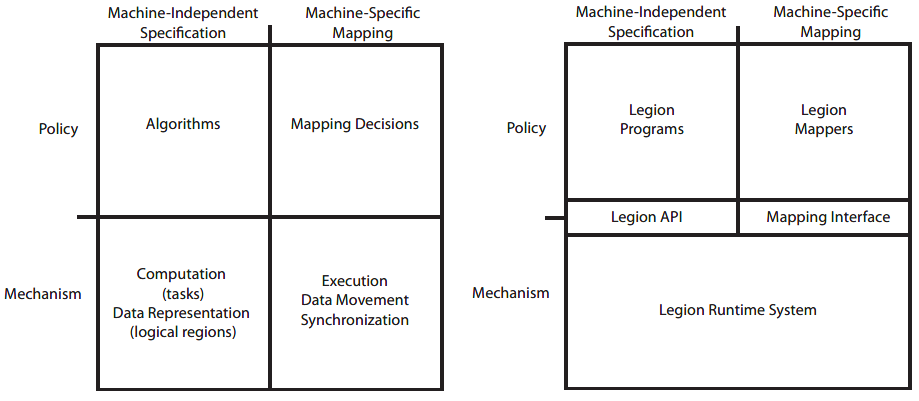
\includegraphics[width=1.0\textwidth]{images/design_principles}
	\caption{Components of supercomputing applications and how they transfer to the Legion Programming System}\label{fig:design_principles}
\end{figure}
Legion's design aims to introduce high level abstractions to manage the increasing complexity faced by scientific programmers. In~\cite{BauerThesis} Legion's developers propose an abstract view of scientific applications as being composed of four primary components divided along two axes (cf.\ Figure~\hyperref[fig:design_principles]{\ref{fig:design_principles}}). On the horizontal axis they distinguish between the machine independent code and the code necessary for specifying machine specific operations. On the vertical axis they differentiate between the code that specifies how an application should be executed (Policy) and the code used to realize this policy (Mechanism). Legion’s goals are:
\begin{itemize}
\item To \textbf{decouple mechanism from policy}, by providing abstractions for developers to specify the applications policies. Therefore writing on the one hand code for the algorithms used and on the other hand code how those computations and data should be mapped to a target hardware. Legion provides the implementation of these abstractions (mechanism)

\item To \textbf{decouple specification from mapping}, by enforcing a strict seperation between machine independent application code and the machine specific code, that describes the mapping. This allows to retarget an application to another architecture without rewriting the program, but just the mapping code. Just as it would be possible to change the used algorithms and kernels without the need of reimplementing data movement, synchronization and scheduling routines.
\end{itemize}

\subsection{Programming Model}\label{sec:programmingModel}
Legion's programming model puts a strong emphasize on sequential semantics. Meaning that programs, which can be executed in parallel with Legion should be readable like a sequential implementation of the problem. This is made possible, because all parallelism is extracted automatically by the Legion runtime. Therefore it is not necessary to mix code describing the program's policy with code that explicitly describes parallelization, communication or synchronization schemes. Legion's approach of implicit parallelism results in far less cognitive load compared to explicit approaches like for example MPI. Legion is designed from the ground up to make dynamic decisions about mapping and data placement during runtime. Computing those decisions introduces a certain overhead, that can be hidden by the runtime if processors run idle while waiting for computations that are still running. Therefore Legion is throughput oriented, meaning that if tasks are long running enough communication latencies and runtime overheads can be effectivly hidden.

This is made possible by the use of specifying the properties of the data used in the application. Possible data properties include: The organization of the data, its partitioning, the access priviliges tasks have on the data and the coherence with which they operate on it. With this information provided by the programmer, Legion is able to extract the implicit parallelism and issue the necessary data movement operations in accordance with the declared properties.

Last but not least, Legion allows a certain control over how the application is mapped onto different architectures through its mapping interface. Users can implement their own work stealing strategies to distribute the workload between different processing units present in the architecture. All code implementing mappers is completely seperated from the application code and can not affect program correctness. This allows for an easy porting of applications to new architectures and environments.

The three fundamental abstractions in the Legion programming model --- logical regions, partitions and (trees of) tasks. --- will be described in the following sections.

\subsubsection{Logical and Physical Regions}\label{sec:logicalRegions}
Regions are the fundamental datatype in the Legion programming model.
They are the abstraction that decouples the description of data from any mapping of the data in the hardware.
Therefore Logical Regions have no implied location or placement in the memory hierarchy. They are not allocated immediately in memory but only when a task with write privileges is invoked (e.g.\ for initalization) and may be moved as necessary between nodes or even exist in partial or full copies on multiple nodes.
The definition of Logical Regions is inspired by relational databases and the work to represent data structures through relational algebra and functional dependencies presented in~\cite{hawkins2011data}. 
But Legion does not aim to reimplement a relational database system, therefore support for relational algebra is limited. 
A more detailed description of relational operations, which can be performed on regions will be provided in Section~\ref{sec:partitions}. 
To get a first grasp on the concept of Regions one should imagine the data as being stored in a table with rows and columns.

To describe the rows of logical regions, Legion uses so called index spaces, which define the keys to a region. Legion currently supports two types of index spaces: structured index spaces to represent data that should be accessed with a collection of dense keys, like arrays or N-dimensional Cartesian grids; and unstructured index spaces to represent data that should be accessed by a arbitrary collection of keys, like most pointer data structures. For now Legion only supports structured index spaces for one, two and three dimensions and unstructured index spaces in the form of a fixed length collection of (mapping independent) pointers. In the future the implementation of more types of index spaces is planned, to represent different sparsity patterns of data, for example for sparse matrix representations.

To describe the columns (fields) of logical regions, Legion uses so called field spaces. A field space describes and names all fields available in a logical region, which can consist of plain old data types and compound types. Field spaces as a feature of Legion were introduced in 2014 and a detailed description can be found in~\cite{ExtendingLogicalRegions}. Field spaces decouple the policy of describing what constitutes a field from the mechanisms how this field will be implemented and used.

With the introduction of the concepts of index spaces and field spaces we can define a region as the crossproduct of an index space and a field space: Each field $f \in F$ has a type $T_f$ and a pair $\left< i,f \right>$ where $i \in I$ and $f \in F$ is sufficient to uniquely identify an entry of type $T_f$ in the region.

\subsubsection{Partitions}\label{sec:partitions}
Logical Regions can be partitioned to name different subsets of the data in the region that will be used by different computations. This creates so called sub-regions, that form a hierarchical relationship with their original region, thus forming a region tree.
Again, partitions and the resulting sub-regions are not a form of physical representation of the data in the memory hierarchy, but just representations of different views on the same underlying dataset. Let's take for example a one-dimensional indexspace of $1..60$ and a field space just consisting of one boolean field. The resulting logical region would be similar to an array of booleans with 60 elements. It would be possible to form an equal disjoint partitioning of this array into six sub-regions á 10 elements or three sub-regions á 20 elements. It is not necessarily required to duplicate any physical data for this, instead the programming system will figure out necessary data operations based on the data dependencies in the source code.

Partitioning in Legion is done via so called \emph{colorings}\@. Colorings describe the partitioning of an index space by mapping a ``color'' to a set of points in the respective index space. For unstructured index spaces this means mapping colors to sets of pointers and for structured index spaces mapping colors to one or more groups of Cartesian points. The analogy of coloring for this operation stems from the possibility of visualizing the process as colorizing parts of the data structure as seen in Figure~\hyperref[fig:partitioning]{\ref{fig:partitioning}} presented in~\cite{DependentPartitioning}, where two different partitionings of a Graph data structure are performed. First into a disjoint and complete partitioning of circuit subpieces rn\textsubscript{n} --- meaning that no field is part of more than one subregion and every field of the parent region is in one of the subregions --- and second in an incomplete (surjective) and aliased partition of ghost regions rg\textsubscript{n}.

\begin{figure}[htb]
	\centering
	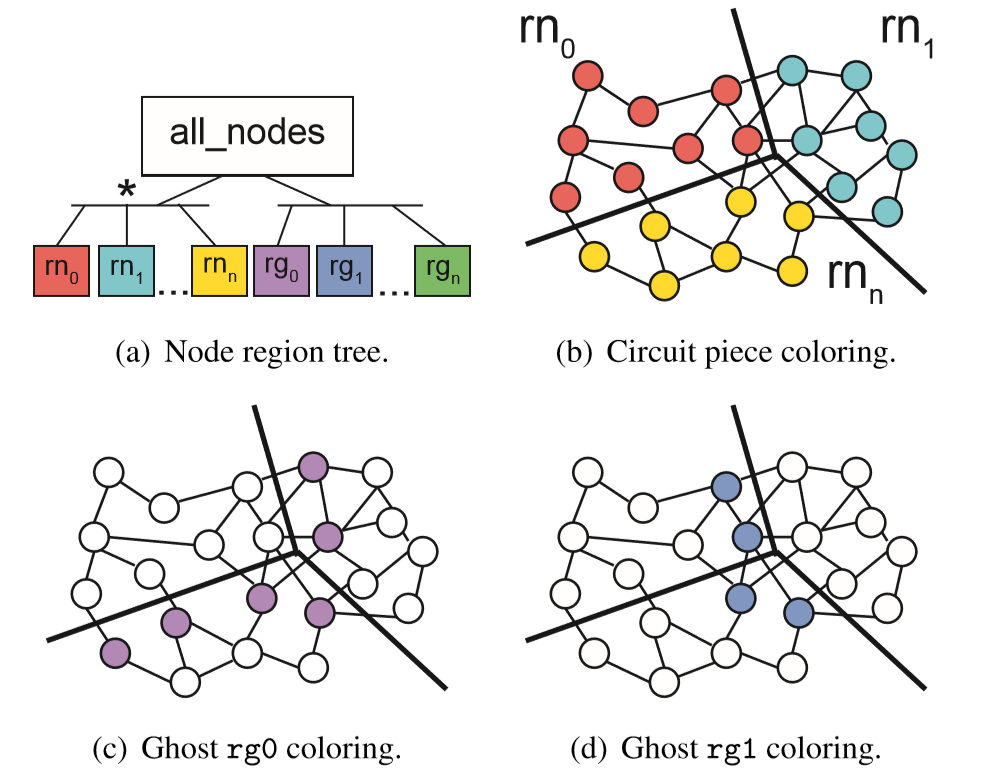
\includegraphics[width=0.8\textwidth]{images/partitioning}
	\caption{Two different partitions of a Graph data structure. One disjoint and complete, the other aliased an incomplete.}\label{fig:partitioning}
\end{figure}

Dependent Partioning is one of the most recent feature additions to Legion, presented 2016 in~\cite{DependentPartitioning}, with a first working implementation released in 2017. It introduces a new distinction between \emph{Independent Partitions}, meaning partitions created from scratch, and \emph{Dependent Partitions}, which are derived from independent partitions using a small set of \emph{dependent partitioning operations}. Those partitioning operations are based for one on set operations and second on reachability via pointers. Available operations include Union, Intersection, Difference, Image and Preimage, the two last corresponding to the mathematical definitions of image and preimage:
\begin{align}
	\label{eq:imagePreimage}
	\nonumber & \text{For a function } f\colon X \to Y \text{ and } M \subset X                 \\
	          & f(M) := \{ f(x) \mid x \in M\} \text{ describes the image}                      \\
	\nonumber                                                                                   \\
	\nonumber & \text{For a function } f\colon X \to Y \text{ and } M \subset Y                 \\
	          & f^{-1}(M) := \left\{x\in X\mid f(x)\in M\right\} \text{ describes the preimage}
\end{align}
In short the Image and Preimage operations compute a partition forwards or backwards through a pointer field inside a region as shown in~\hyperref[fig:image_preimage]{\ref{fig:image_preimage}}.

\begin{figure}[htb]
	\centering
	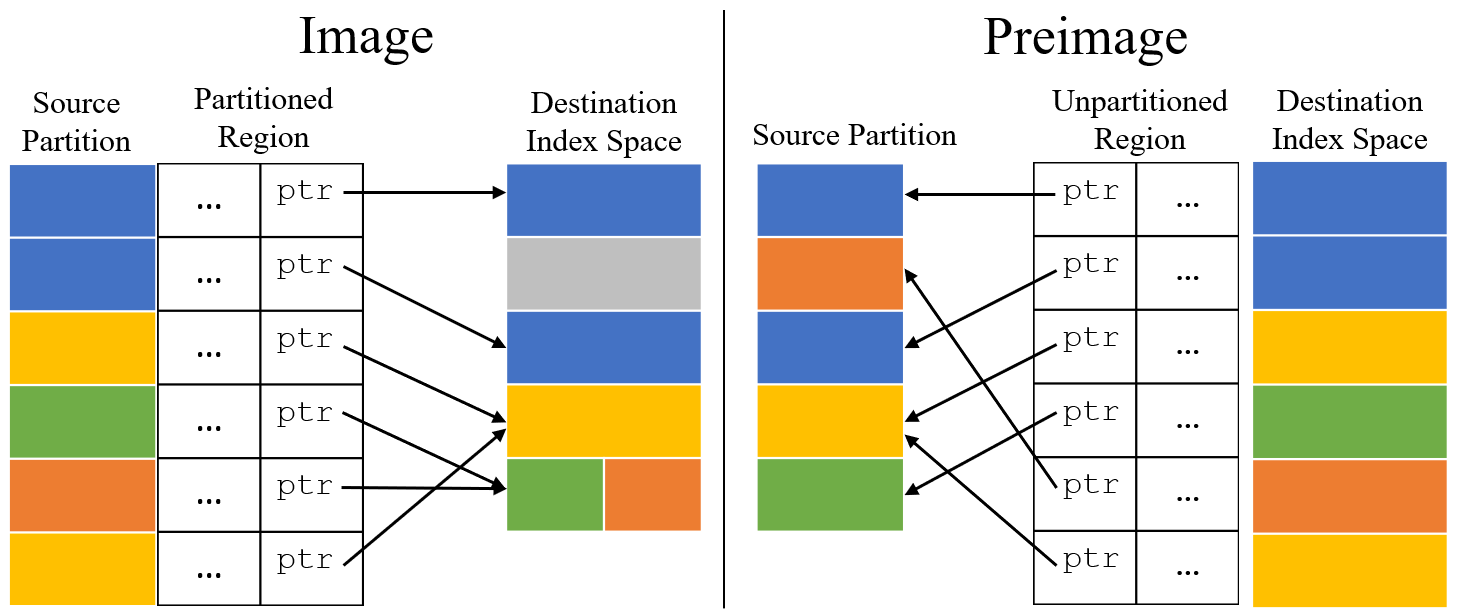
\includegraphics[width=0.9\textwidth]{images/image_preimage}
	\caption{Dependent Partitioning via Image and Preimage operations}\label{fig:image_preimage}
\end{figure}

\subsubsection{Tasks}\label{sec:tasks}
A task is the fundamental unit of control in Legion and can take two kinds of arguments: Parameters which are passed by value and logical regions to operate on.
A unique property of the Legion Programming Model is the absence of a heap abstraction that could be implicitly accessed by any computation. Instead Legion requires its task to explicitly describe on which regions they operate on (the task's \emph{region requirement}) and the way how they want to access those regions (the task's \emph{privileges}). 
Available privileges include \emph{Reads}, \emph{Reads-Writes} and \emph{Reduces}. 
The reduce-privilege requires the specification of a commutative and associative reduction operator.
Regent, the programming language implementing Legion's Programming Model, currently lists the availabale operator as $+, *, -, /, min \text{ and } max$.\footnote{Why the Regent Reference also lists operators that are not commutative or associative could not be clarified. 
However Regent is technically implemented as a language extension of the low-level system programming language Terra~\cite{Terra}, those operators being a valid argument for the reduce-keyword could therefore be a result of the limitations in Terra's language extension syntax.} 
There exists an additional privilege \emph{Writes-Discards}, which is currently only documented in the glossary of  the Legion runtime. 
This privilege allows a task to communicate its intent to overwrite the specified field(s) without reading them and thus allowing the runtime to perform certain optimizations associated with removing unnecessary data movement operations.

Legion's model of computation is a tree of tasks. This means tasks are free to spawn sub-tasks with an unlimited level of depth, which sets it apart from the traditional SPMD programming model usually associated with programming supercomputers. However sub-tasks are only allowed to access logical regions, that are accessed by its parent task and only within a non-strict subset of the privileges specified by its parent task. This is called the \emph{containment property} and is an important constraint used by the runtime scheduler. In~\cite{BauerThesis} it is noted that this leads the Legion Programming Model to be a hybrid between functional and imperative programming models: Between tasks Legion behaves like a functional model, with tasks only accessing subsets of the data their parents are able to access. On the other hand tasks are composed of statements that mutate the state of logical regions like imperative programs manipulate data on one or more heaps.

Tasks are Legion's unit of parallel execution. All sub-tasks are launched asynchronously and it is the runtime's responsibility to maintain sequential program order semantics for those tasks. Legion's runtime allows sub-tasks to run in parallel if they are \emph{non-interfering} on their logical region arguments. Through the automatic discovery of independent work within a program, Legion is able to not only hide the large latencies present in supercomputer systems, but also the latency associated with its dynamic analysis --- given the parallelised tasks are long-running enough. The promise that all tasks are launched asynchronously while at the same time Legion guarantees the sequential program order semantics of an application is called the \emph{Deferred Execution Model}. In essence this execution model allowes Legion to execute workload or communicate data between nodes somewhere between the point in time that its dependencies are fulfilled and the point in time when another operation depends on it. Therefore, a well written Legion program is able to use idle resources or hide latencies by executing operations at a self-chosen and possible favourable point in the execution of the program.

An important aspect of tasks in Legion are \emph{Task Qualifiers} which provide additional information what a task will or will not do during runtime.  There exist three task qualifiers that can be associated with a task: \emph{inner}, \emph{leaf} and \emph{idempotent}. Tasks are considered inner, if they are not at the end of a branch in the task tree. Inner tasks are not permitted to access the logical regions they have privileges for, but are only able to launch subtasks and pass their privileges on to them. Inner tasks can start execution even before their data dependencies are fulfilled, as data access can only occur at a deeper level. This is an important property to discover additional task parallelism generated by inner tasks. Leaf tasks are at the end of a branch in the task tree, meaning they launch no other sub-tasks. Leaf tasks are not allowed to perform any Legion operations like creating or partitioning regions. They usually are sequential programs and generally the location of the heavy computing performed by an application. Thus, leaf tasks should be optimized for latency and not throughput, meaning they should finish execution as fast as possible. Idempotent tasks have no side-effect except on logical regions. This means for example they do not write to files or print output. In general nearly all tasks in a Legion application should be idempotent. It is important to note, that the Regent programming language automatically infers task qualifiers. Only source code targeting the Legion Runtime API directly needs to specify those explicitly.

Last but not least Legion allows the programmer to specify \emph{Task Variants}, by registering multiple functionally equivalent implementations of the same task. An Idea similar to a feature of Sequoia~\cite{sequoia}. This allows applications to adjust algorithms and physical data layout depending on the target architecture and by using Legion's mapping API spevify different task variants depending on the available processing units on a node. However this feature is currently not implemented in Regent.

\subsection{The Legion Runtime}
Legion's main component is the Legion Runtime system, which implements the \emph{deferred execution} model. Implementing Legion as a runtime system enables the dynamic properties of the programming model and is a fitting solution of the second problem with which scientific computing is confronted today: The increasing amount of dynamism in hardware and software. The runtime system is implemented in C++, which should make it easy for existing applications to be ported as developers are already accustomed to the language and only need to adapt to the new programming model. Furthermore, C++ was choosen because it was evaluated as a common target for the compilers of Domain Specific Languages, which could implement the Legion Programming Model.
\begin{figure}[H]
	\centering
	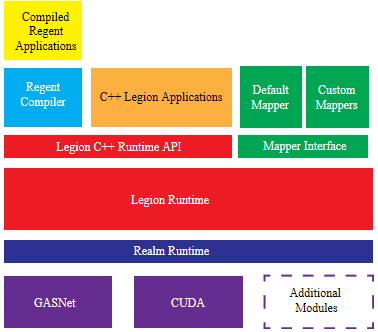
\includegraphics[width=0.6\textwidth]{images/system_architecture}
	\caption[Caption for LOF]{Architecture of the Legion Programming System\footnotemark}\label{fig:syste_arch}
\end{figure}

% TODO: This footnote has to appear on the same page as the figure system_arch
% https://tex.stackexchange.com/questions/10181/using-footnote-in-a-figures-caption
\footnotetext{This figure was taken from the offical Legion Project website:\newline \url{legion.stanford.edu/overview}}

Figure~\hyperref[fig:syste_arch]{\ref{fig:syste_arch}} shows the complete system architecture of Legion. Not shown is the C-wrapper for the Legion C++ Runtime API, that is used by Regent.
 Important to note is the divide between Legion applications seen above the Legion Runtime API and the mapping interface (green blocks). 
This is the concrete representation of Legion's goal to decouple machine independent code from hardware specific mappings. Currently custom mappers have to be implemented in C++ regardless of the language used to implement the machine independent Legion Application. 
It is the responsibility of the runtime to mediate between the machine-independent application specifications and the decisions provided by the mapping objects (compare Figure~\hyperref[fig:design_principles]{\ref{fig:design_principles}}).

The Runtime system is further divided into a high-level runtime (Legion) and a low-level runtime (Realm). The high-level runtime supports the C++-interface for writing Legion applications. However, C++-Legion applications have to abide fully to the already presented programming model;
meaning they are not allowed to use dynamic memory allocations and have to use logical regions instead. Additionally, tasks are only permitted access to data in regions they request privileges for and all sub-tasks must be launched via the runtime interface. 
The Legion Runtime mediates between the mapper object and the legion application by directing decision requests for task assignments and physical instances through to the mapping interface and carrying out the results on the target architecture.

A description of the low-level runtime Realm is beyond the scope of this thesis. 
An overview can be found in \cite{Realm} and a detailed description in \cite{TreichlerThesis}. 
Realm provides the primitives for orchestrating computation, data movement, and synchronization. 
This means launching tasks on specific processors remote or locally, allocation and freeing of physical memory, copy and reduction operations between physical instaces and synchronization. One of the most important design decisions of Realm is, that all those primitives are implemented in a non-blocking fashion. 
Low-level runtime operations return \emph{events}, that name a time at which the operation will be completed and are able to take those events as preconditions for the execution of operations. 
This design allows the high-level runtime to construct directed acylic graphs (DAG) --- that describe the program execution and the extracted possible parallelism --- and hand this off to the low-level runtime as a stream of event-dependent operations for scheduling. How those DAGs are constructed by the Legion Runtime System will be described in Section~\ref{sec:dependency}.
It is the responsibility of the low-level runtime to use the information computed by the high-level runtime to find long-running tasks, that enable the hiding of communication or synchronization events. 
Additionally, the low-level runtime increases Legion's portability. 
It provides an abstraction layer between Legion's complex procedures, implemented in the high-level runtime and various hardware interfaces. 
It is the hope of the Legion developers, that future architectures will only require a reimplementation of the low-level runtime to port the whole programming system to them.

\subsubsection{Mapping}\label{sec:runtimeMapping}
The mapping interface provides the means for Legion application developers to directly controle how their programs are mapped onto the target hardware. It is implemented as a call-back model. Whenever a mapping decision needs to be made, the runtime queries a local instance of the mapper object to perform the decision.
Mapping objects have a direct access to a singleton called the machine object. The machine object is an interface, which provides information about the underlying hardware on which the application is executed. This machine object is provided by the low-level runtime directly to the mapper. It holds information about the available processors and memories, as well as their respective latencies and bandwidths. Currently the machine object is static and cannot be changed during the execution of an application. A planned future feature addition to Legion would allow the machine object to change, depending on changing hardware states, as for example the failure or addition of nodes in a supercomputer.

To dive deeper into the Legion's ability to be executed in a distributed environment it is important to note, that an instance of the runtime is created on every node in executing machine, while mapper objects are instantiated in a one-to-one fashion per processor on a node. By having seperate mappers for each processor it is possible to avoid sequential bottlenecks, as tasks mapping on different processors will never conflict over a common mapper object.

A detailed description of the mapping interface and which methods a user may or may not need to implement is given in Section~\ref{sec:mappinginterface}.

\subsubsection{Program Execution Framework}
As described in Section~\ref{sec:tasks}, to adhere to the Legion programming model means to write programs as a tree of tasks, which operate on logical regions. To execute these trees, Legion relies on a task pipeline, similar to out-of-order pipelines implemented in hardware architectures. Legion adapts the fundamental idea of out-order-order pipelines and applies them on the coarser granularity of task execution in distributed environments. In~\cite{LegionPaper}~and~\cite{SlaughterThesis} this is called a \emph{software out-of-order processor} (SOOP), however this name is never used again in later publications. A way to think about this concept is to envision the tree of tasks as a hierarchical collection of streams of tasks with the execution of a task generating new streams of sub-tasks. As multiple instructions can be in different stages of execution at the same time in a pipelined processor architecture, Legion tasks can be in different stages of the execution pipeline at the same time. The main difference being, that hardware instructions are not able to generate new instructions, while in Legion, the execution of a task can potentially spawn new streams of sub-tasks, which have then to be executed.
\begin{figure}[htb]
	\centering
	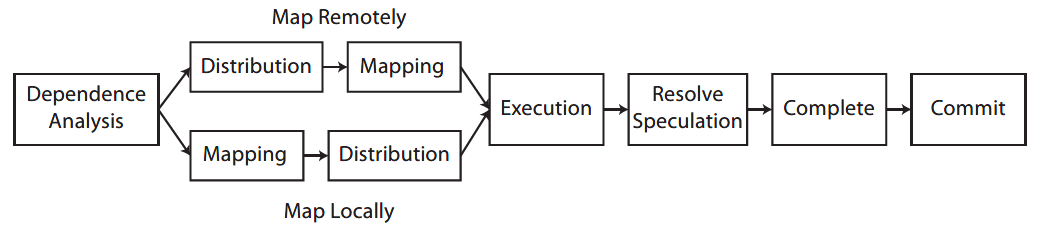
\includegraphics[width=0.9\textwidth]{images/task_pipeline}
	\caption{Legion Runtime Task Pipeline}\label{fig:pipeline}
\end{figure}
Figure~\hyperref[fig:pipeline]{\ref{fig:pipeline}}, as shown in~\cite{BauerThesis}, depicts the stages of the Legion runtime task pipeline. Every task progresses these stages in order, but it is possible for the runtime to reorder tasks, if they are determined to be non-interfering. For example to temporarily halt a task's pipeline to wait for other tasks finishing stages.

The first stage is the dependence analysis --- described in greater detail in Section~\ref{sec:dependency} --- which is computed in the sequential order in which the tasks are issued to the runtime. Once a task has all its dependencies fulfilled, meaning the tasks it depends on have finished the mapping phase of the pipeline, it can be mapped either locally, where it originated or remotely, meaning on another node.
The execution stage is similar to the execution of instructions in hardware processors. Instead of assigning instructions to execution units, tasks are assigned to processors, which then executes the task.
After the execution any speculations have to be resolved. 
This is due to Legion being capable of speculative execution by predicating tasks (again a concept similar to speculative execution in modern processor architectures).
If a task was predicated and the mapper choose to speculate on the predicated value, this stage checks for the results of the speculation to hold true or not. 
This means if the speculation was incorrect, the task has to be reexecuted or the results of the task must be undone. 
Furthermore, speculation can impact dependent tasks and all tasks with dependences on the mis-speculated task must also be rolled back. For tasks without predicates, this stage performs no work at all. The next-to-last stage ``completion'' is necessary because of Legion's deferred execution model. It is possible that a task finishes the execution stage of the pipeline, while its sub-tasks have yet to be executed. At this stage a task waits for all its child tasks to reach the completion stage. Once this condition is fulfilled, the task has been correctly executed and may propagate information back. Tasks that depend on the completion of this task can now start execution. The last stage exists for resilience purposes. In the commit stage a tasks' metadata, like task id or region requirements are reclaimed. A task can only be commited once the runtime can be certain that no roll-back or reexecution of the task will ever be necessary.

To allow for a viable implementation of this execution pipeline Legion relies on the fact that a task needs only to consider other tasks within the same stream, meaning originating from the same parent, when progressing through the stages of the pipeline. This is due to the constraint of tasks being only allowed privileges on a subset of the regions and fields privileges its parent holds introduced in Section~\ref{sec:tasks} as the \emph{containment property}. This property is sufficient to prove that, if two tasks $t_1$ and $t_2$ are non-interfering, then all sub-tasks of $t_1$ will be non-interfering with all subtasks of $t_2$. A full proof of this theorem can be found in~\cite{LanguageSupport}. This theorem permits the runtime to use a hierarchical scheduling algorithm, which allows many tasks to traverse the task pipeline in parallel on different nodes. Also, since all tasks in a common stream originate on the same node, no inter-node communication is necessary for performing the dependency analysis.

\subsubsection{Dependency Analysis}\label{sec:dependency}
The first stage of the Legion task pipeline
computes which tasks are interfering and therefore must have dependencies.
A naive implementation would perform pairwise tests for non-interference between subtask and all tasks launched before it from the same parent. For a stream of N tasks this would require $O(N^2)$ tests to be performed. In practice N is a sliding window reflecting tasks that have yet to complete in a particular stream of tasks S.
As a asymptotically superior algorithm for dependency analysis is unlikely to be found, Legion aims to reduce the constant factors of the dependency analysis.
To achieve this goal it is important to first define when tasks do not interfere with each other. In~\cite{BauerThesis} three disjunct conditions of non-interference are given:
\begin{itemize}
	\item \textbf{Region Disjointness:} The logical regions in the two region requirements of the tasks are disjoint (no shared rows).
	\item \textbf{Field Disjointness:} The sets of fields requested by the two region requirements of the tasks are independent (no shared columns).
	\item \textbf{Privilege Non-Interference:} Either both region requirements of the tasks are requesting read-only privileges, or both region requirements are requesting reduction privileges with the same reduction operator.
\end{itemize}
As proving one of these three conditions is already sufficient for proving non-interference, they can be tested in any order. If one test should be successful, any remaining tests can be skipped. Through experimentation the Legion developers chose the order of region disjointness, field disjointness and privilege non-interference as the one that minimizes the number of tests performed the most.

This means that the Legion developers identified region disjointness as the most effective test for task non-interference. As mentioned in Section~\ref{sec:partitions} regions and their respective sub-regions form a tree. The use of a region tree data structure is crucial to make the test for region disjointness inexpensive to compute. To perform the dependency analysis for a sub-task $T$ in stream $S$ it is necessary to identify all other tasks that come before $T$ in $S$ that interfere with at least one region requirement of $T$. Thus a seperate analysis for each region requirement of $T$ has to be performed. A tree traversal algorithm is used to traverse the region tree forest for each region requirement of $T$ and identify tasks from $S$ that are not disjoint on region usage. First a path from the logical region requested by the task, to the logical region on which its parent task own privileges is computed. This path is guaranteed to exist because of the containment property introduced in section~\ref{sec:tasks}. This path allows an easy identification of all nodes in the region tree that must be visited throughout the test. The set of nodes includes all nodes along the computed path, as well as any sub-trees of nodes along the path that may contain interfering nodes (remember, that region partitions can be aliased). To deduce if the region usage of a task is interfering with the region usage of another task on this set of nodes it is necessary to keep track of the tasks that use a respective region/node. An effective solution to this is, that each task in $S$, on which this dependency analysis is performed registers itself as a \emph{user} of the region tree nodes for each logical region it requests privileges on. Such a user record stores information about the respective task, its requested fields, privileges and coherence. As mentioned earlier, only non-completed tasks in $S$ have to be considered for the dependency analysis. Therefore it is possible to remove user records of tasks that already finished execution and also user records for which it can be proven, that no transitive dependences exist. The resulting set of nodes including the user records for each node is also the basis for the remaining two tests of non-interference. In the end the result of the dependency analysis is stored as a \emph{dynamic dependence graph}.

This is a directed acylic graph in which nodes represent operations like sub-tasks or explicit copy operations, and in which edges represent the dependences that result from interfering region requirements. To ensure for a task $T$, that all dependences and data movement operations have been determined correctly, it is necessary that $T$ is only allowed to be mapped, when all the other tasks in the dynamic dependence graph on which $T$ has a dependence have been mapped. Recall that logical regions are abstract from their physical representation, thus it is crucial to wait for this condition to be fulfilled, so that $T$ is able to access the correct version of meta-data stored about the physical state of the region tree forest. Only the task can proceed to the second stage of the execution pipeline (mapping). The physical dependence analysis uses a similar tree traversal algorithm as the logical dependence analysis. What is the major difference is the desired result. Instead of generating a dynamic dependence graph, the purpose of the physical dependence analysis is to issue the appropiate operations to the Legion low-level runtime. This means the physical dependence analysis makes several queries to the mapper during its execution. Another difference is, that while it was necessary for the tasks in a given stream $S$ to perform their logical dependency analysis in order, to ensure the corrrect storage of user records, it is possible for several tasks, for which all mapping dependencies have been fulfilled, to perform their physical dependency analysis in parallel.

\subsection{Debugging and Profiling}\label{sec:profDebug}
Legion supports some useful execution flags to assist developers in debugging. First and foremost Legion can be built in debug mode by using \inlinecode{Bash}{DEBUG=1} with the Makefile infrastructure. This enables additional checks and assertions to produce meaningful error messages.

Further Legion can freeze if it reaches an error, like an assertion failure or segmentation fault. This can be turned on by setting the environment variable \inlinecode{Bash}{LEGION_FREEZE_ON_ERROR=1} before launching a Legion application. When encountering an error, the application will then freeze and the process ID and node will be printed to console. This allows to attach a debugger like gdb to the frozen process.

Legion features a type system, described in~\cite{LanguageSupport}, to statically verify that region accesses follow the privileges declared by the tasks. However, these guarantees are only available for Legion applications written in Regent. For applications targeting the runtime interface directly it is possible to dynamically verify if tasks violate their declared privileges. To enable this feature it is neccesarry to add the \inlinecode{Bash}{-DPRIVILEGE_CHECKS} flag to the list of compile time flags specified by the \inlinecode{Bash}{CC_FLAGS} variable inside Legion's Makefile.

Another safty feature provided by Legion's type system, that is not available when targeting the runtime interface directly are Bounds Checks, to verify if all memory accesses fall within the bounds of the logical region requested by a task. To insert dynamic bounds checks during the application execution the \inlinecode{Bash}{-DBOUNDS_CHECKS} flag has to be added to the \inlinecode{Bash}{CC_FLAGS} variable inside Legion's Makefile.

For complicated coloring schemes, it is possible to execute a Legion program with the \inlinecode{Bash}{-lg:disjointness} flag. This performs disjointness checks on all partitions, even those that were produced with methods that are meant to result in disjoint partitions. This helps application developers to ensure that they don't pass incorrect disjointness information to the runtime system.

Additionally, the Legion Programming System currently comes with two tools for debugging and profiling Legion applications either targeting the C++ runtime directly or written in Regent. Both are currently in the process of being merged together. Therefore, there is an overlap in functionality between the two.

\textbf{Legion Spy} is a tool to visualize the task dependencies generated by a Legion application. Simply put, it generates the dynamic dependence graph mentioned in Section~\ref{sec:dependency}. Legion Spy features two execution modes to achieve this: First it includes a second implementation of Legion's dependence analysis algorithm to verify the runtime itself, by cross-checking its results against dependency data captured from a program run. This can be an expensive operation and needs the additional compile flag \inlinecode{Bash}{CC_FLAGS=-DLEGION_SPY}. Second it can generate a dependency graph on its own as a sanity check to confirm that an application features the dependencies and tasks a developer would expect. For this it is sufficient to execute a Legion application with the flags \inlinecode{Bash}{-lg:spy -logfile spy_\%.log} and run the post-processing script \inlinecode{Bash}{legion_spy.py} on the generated logfiles. One logfile per node will be generated.
The post-processing script is capable of generating a dataflow graph with \inlinecode{Bash}{-d} to visualize the order in which data is processed by the defined tasks and an event graph \inlinecode{Bash}{-e}, which illustrates tasks and their dependencies. Additional information like field names can be included by adding the \inlinecode{Bash}{-z} flag.

\textbf{Legion Prof} is a profiling tool for Legion applications. Currently it is able to interprete data generated by Legion Spy to show dependencies for a selected task. To use the profiler, a Legion application must be run with \inlinecode{Bash}{-lg:prof <N> -lg:prof_logfile <file>}, where N is the number of nodes to be profiled. The post-processing script \inlinecode{Bash}{legion_prof.py} is used to generate a \inlinecode{Bash}{legion_prof} subdirectory from the logfile.
In this directory the file index.html allows the user to view the profiling data in a webbrowser. Because of compatibility issues with modern webbrowsers it is advised to run a local web server to access this file, instead of opening it directly.


\subsection{The Legion Mapping Interface}\label{sec:mappinginterface}
In Section~\ref{sec:runtimeMapping} it was mentionend that the high-level runtime uses local instances of a mapper object to perform mapping decisions. As described in Section~\ref{sec:solutions} it is the goal of the Legion Programming System to allow developers to provide machine-specific mapping instructions decoupled from the machine-independent program specifications. This functionalty is provided through the Legion Mapping Interface, a C++ interface listed in Appendix~\ref{app:mappinginterface}. Mappers being objects of this abstract class allows them to be stateful and therefore use the results of previous mapping decisions in the process of answering later queries from the runtime. All methods in the interface are declared as virtual, which allows the easy creation of specialized mappers as modification on already existing ones.

Mapper objects are able to query the runtime about the underlying hardware through the machine object singleton already mentioned in Section~\ref{sec:runtimeMapping}. This singleton provides methods for finding all processors and memory locations throughout the entire system, including those on remote nodes. Additionally, it provides information about the kind of processors and memories present. There are three kinds of processors, that are currently recognized by Legion: latency-optimized cores (CPUs), throughput-optimized cores (GPUs) and utility processors (CPU core for performing runtime meta-work). The three most important types of memory recognized by Legion include system memory (DRAM), framebuffer memory (GPU GDDR) and registered memory (memory that can be directly accessed by Network Interface Controllers). Furthermore, the machine object provides information about the latencies and bandwidths present in the architecture by exposing affinity relationships between various processors and memories. A processor-memory affinity exists when the processor is able to read and write directly to a memory. A memory-memory affinity exists whenever there is a direct data movement path between the two memories. For ease of use it is possible to organize these components into collections to map onto instead of mapping to a particular processor or memory directly. 

First of all, the case of a task being mapped locally: Once a task finished the dependency analysis stage of the execution pipeline, it is placed in the ready queue for the mapper that manages the processor on which the task's parent is executing. When tasks are in the ready queue, the mapper is queried through a call to \lstinline{select_tasks_to_schedule} to select tasks it would like to map. The tasks, that are ready to be mapped, are given as an ordered list to this method, with the tasks waiting the longest appearing earlier in the list. The mappper has to mark which tasks it wants to map or choose to not map any tasks. By invoking the \lstinline{map_task} function the mapper object is instructed to create a ranking of memories in which to attempt to place the physical instances of the region requirements of the task. This can be specified on a per-requirement basis. To support the mapper decisions process the runtime provides information for each region requirement about already available physical instances and validity of their fields. 

Furthermore, Legion provides three ways to achieve load balancing. One within a Node, and two options, that also enable inter-node balancing. Early it was mentionend that it is possible to organize processors among other components into collections. If there are several processors of the same kind available in a node, it is possible to organize those in a \emph{processors group}. All processors in the same group share a common task queue. This means as soon as any processor in the group is ready to execute a task, it is able to pull it from the queue, without the need to communicate with other mapper objects. Processors groups are the easiest way to achieve load balancing between processors in a single node, but also the most constrained mechanism provided by the Legion mapping interface. 
The two remaining mechanisms, which also support inter-node load balancing are for either based on a \emph{pull} methodology or on a \emph{push} methodology.

The first one is task stealing, which can be used to actively pull work from one node to an idle one. By calling the method \lstinline{target_task_steal} the runtime is able to query each mapper if it would like to target any other processors in the system for task stealing. Once such a request is made, the runtime sends the necessary messages to the mappers on the remote node. This triggers a call of the \lstinline{permit_task_steal} method of the remote mapper object. The remote mapper object is then able to either allow a task in its ready queue to be stolen from it, or refuse the task stealing. In Legion mapper objects must explicitly allow task stealing, as stealing primarily occurs between nodes and therefore the associated costs, due to data movement, are usually high. Program performance therefore can benefit if mappers are able to refuse to send tasks to other nodes if they should explicitly only use intra-node load balancing. If a task is allowed to be stolen, it's meta-data is moved to the node from which the stealing request originated and the particular task is added to the ready queue of the stealing mapper object. Technically task stealing is also permitted within a node. However processor groups are the more efficient approach to intra-node load balancing. Users, developing a mapper, should therefore avoid implementing inter-node task stealing. At the moment, the default mapper used by Legion does not make use of task stealing. However it is noted in~\cite{BauerThesis} that there should exist a command line flag to enable a randomness based task stealing scheme for the default mapper. The implementation of a more advanced stealing scheme is planned as a future addition to the default mapper.

The second mechanism for inter-node load balancing is the push-based model of mapper communication. To allow advanced load-balancing schemes based on direct mapper communication, the Legion mapping interface provides a mechanism to send arbitrary messages to other mapper objects. A message is defined by a pointer to an untyped buffer and size variable holding the number of bytes to copy. The runtime copies this buffer and transmits it to the target node, where it invokes the \lstinline{handle_message} method of the receiving mapper object. Mappers are permitted to send messages inside every mapper call, including the \lstinline{handle_message} one. An example for the usage of this messaging mechanism given in~\cite{BauerThesis} is an adaptive mesh refinement code, where mappers communicate the load of tasks that they receive after each refinement. Based on this information, each mapper could independently compute a load balacing scheme and determine target processors to offload tasks onto.

To allow mapper objects to determine how their decisions impact the application's performance, the mapping interface features several mechanisms to provide feedback about the actual mapping onto the target hardware. The first way for mappers receiving feedback is through \lstinline{notify_mapping_result} and \lstinline{notify_mapping_failure}. It is possible for a mapping to fail, if for example physical instances of requested regions could not be allocated. In this case the runtime notifies the mapper object, that made the failed mapping decision by invoking \lstinline{notify_mapping_failure}. A task, that failed to map is immediately added back into the ready queue, however this feedback mechanism allows the mapper to record the failed results for use in further mapping decisions. Analogue to notifications about mapping failures, it is possible to request notifications about the success of a mapping decision, by returning a respective boolean value in \lstinline{map_task}, \lstinline{map_copy} or \lstinline{map_inline}. If the mapper object returned true for the mapping decisions, the runtime invokes \lstinline{notify_mapping_result} on a successful mapping.

\subsection{Legion as a target for DSL}
Many of aspects of the programming model described in Section~\ref{sec:programmingModel} are not fully supported when targeting the Legion Runtime API directly. This is because not every aspect of the programming model proposed by Legion can be expressed in C++. This forces the Legion API to expose functionality beyond the logical layer of the programming model. For example, it is the responsibility of the application developer to manage both logical and physical regions in the same application. This means a physical region has to explicitly be unmapped before launching sub-tasks that operate on the corresponding logical region, to avoid data races and consistency problems. Another restriction when using the C++ API exists when a developer wishes to declare an accessor object for a physical instance directly. The application has to explicitly wait for the physical region to be ready. This runs counterwise to the idea of deferred execution but would otherwise not be possible.

As a result the Legion runtime API is first and foremost designed as a target for domain specific languages (DSLs), that wish to implement the Legion programming model. Additionally, there are many aspects of the programming model, that could be managed by the compiler of such DSLs. For example features like task qualifiers discussed in Section~\ref{sec:tasks} or managing the Legion type system, could be hidden from the developer and instead be the responsibility of specialized language compiler. The first DSL to represent a full implementation of the Legion programming model is \emph{Regent}, first published in~\cite{regentPaper} in 2015, three years after the publication of Legion itself.

\section{The Regent Programming Language}

\begin{wrapfigure}{r}{0.30\textwidth}
	\centering
	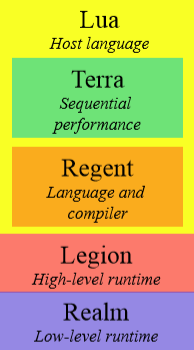
\includegraphics[width=0.25\textwidth]{images/regent_stack}
	\caption{The Regent Stack}\label{fig:regent_stack}
\end{wrapfigure}

Regent~\cite{regentPaper,SlaughterThesis} is a Lua~\cite{lua} embedded language implementing the Legion programming model by providing dedicated keywords and function calls for the declaration of index spaces, field spaces, regions, partitions and task privileges. Technically Regent compiler is implemented using the language extension feature of Terra~\cite{Terra,TerraDesign}. Terra itself is embedded in and meta-programmed by Lua. Terra is a statically-typed and just-in-time compiled language aimed at high-performance computing. One of the specified use cases of Terra is its ability to provide an embedded JIT-compiler for domain-specific languages written in Lua/Terra. Terra uses LLVM~\cite{lattner2002llvm} as a backend and claims to achieve performance compareable with C code compiled using the llvm-toolchain. Additionally, using LLVM's intermediate representation allows Terra and Regent functions to call and link against native C libraries. The C interoperability also allows the use of Legion features not yet implemented in Regent by calling Legion runtime functions directly through a C wrapper.

\subsection{Representation of Legion's Programming Model}
Many of the aspects of the Legion programming model described so far, need to be expressed very explicitly when writing code that targets the C++ runtime directly.
For example, it is necessary to declare region requirements directly by using \lstinline{RegionRequirement} in the Legion API.
A region requirement has to be given as a parameter to a \lstinline{TaskLauncher} or \lstinline{IndexLauncher} instance and the task has to be explicitly launched by calling the \lstinline{execute_task} method of the runtime object.
This means that the declaration of a task and a subsequent launch can involve many lines of code, that are hard to identify as a simple function execution, as can be seen in Listing~\ref{lst:pennant_legion}. Additionally, the C++ API is unable to provide a full abstraction from the physical instances of Legion's region.
A developer has to manually unmap a physical instance before launching a task on its corresponding logical region. Special \lstinline{Accessor} types must be used to actually access the data contained in a physical instance, that make heavy use of C++ templates.

\lstset{
	captionpos=b,
	language=C++,
	basicstyle=\scriptsize,
	numbers=left,
	numberstyle=\tiny,
	columns=fullflexible,
	stepnumber=1,
	escapechar=\#,
	keepspaces=true,
	literate={<}{{$\langle$}}1 {>}{{$\rangle$}}1,
	}

\begin{lstlisting}[frame=single,label={lst:pennant_legion},
		caption={Excerpt from PENNANT~\cite{ferenbaugh2015pennant} main simulation loop in Legion C++ API as presented in~\cite{SlaughterThesis}.}]
Domain domain = Domain::from rect<1>(
	Rect<1>(Point<1>(0), Point<1>(conf.npieces - 1)));
IndexLauncher launcher1(ADV_POS_FULL, domain, TaskArgument(), ArgumentMap());
launcher1.add_region_requirement(
RegionRequirement(points_all_private_p, 0 /#$\star$# identity projection #$\star$#/, 
	READ_ONLY, EXCLUSIVE, points_all_private));
launcher1.add_field(0, PX0_X);
launcher1.add_field(0, PX0_Y);
launcher1.add_field(0, PU0_X);
launcher1.add_field(0, PU0_Y);
launcher1.add_field(0, PF_X);
launcher1.add_field(0, PF_Y);
launcher1.add_field(0, PMASWT);
launcher1.add_region_requirement(
RegionRequirement(points_all_private_p, 0 /#$\star$# identity projection #$\star$#/, 
	READ_WRITE, EXCLUSIVE, points_all_private));
launcher1.add_field(1, PX_X);
launcher1.add_field(1, PX_Y);
launcher1.add_field(1, PU_X);
launcher1.add_field(1, PU_Y);
launcher1.add future(dt);
runtime->execute_index_space(ctx, launcher1);
\end{lstlisting}

Furthermore, the C++ API only allows partitions of index spaces. This means, to create subregions of a logical region, the index space of the parent region is partitionend as wished and the resulting ``sub-index-spaces'' used to access the subregions. In Regent this distinction between the index space and the corresponding region during partitioning is more or less irrelevant. Partitioning operations are usually applied to regions without the need to think about how this could affect the index space.

When handling trees of tasks in the Legion C++ API it is the developer's responsibility to reduce runtime analysis overhead by using correct task qualifiers when launching subtasks (such as \emph{leaf task}). Task Qualifiers are completely hidden from the user in Regent and exclusively managed by the compiler. Additionally, a developer targeting the C++ runtime directly has to distinguish between the possible return types of issued tasks. Tasks can produce a result without blocking their parent task by returning a future of the value. Those futures can also be passed to other subtasks without blocking the issuing task. On the other hand a developer is free to use immediate results in the C++ API with the cost of possible blocking program execution. This distinction between futures and immediate results is also completely hidden from the user in Regent.

To summarize, it can be said that Regent tries to solely expose the logical aspects of the programming model to the user. Features like physical instances, task qualifiers and futures are handled by the compiler itself. Therefore, Regent achieves the goal of full sequential semantics with tasks acting like functions and regions acting like arrays of structs. An example of this can be seen in Listing~\ref{lst:regent_example}

\lstdefinestyle{regent}{
  language=[5.1]Lua,
  basicstyle=\ttfamily,
  morekeywords={where,task,fspace,var},
  keywordstyle=\color{magenta},
  stringstyle=\color{blue},
  commentstyle=\color{black!50}
}
\lstset{
	captionpos=b,
	style=regent,
	basicstyle=\scriptsize,
	numbers=left,
	numberstyle=\tiny,
	columns=fullflexible,
	stepnumber=1,
}
\begin{lstlisting}[frame=single,label={lst:regent_example},
	caption={A simple example of Regent's syntax}]
import "regent"
-- use terras C interoperability to get access to stdlib.h
local c = terralib.includec("stdlib.h")

-- declare a field space
fspace point_fs {
  x : double,
  y : double,
}

-- define a task
task init(input_lr : region(ispace(int1d), point_fs))
where 
	writes(input_lr.{x, y}) 
do
  for i in input_lr do
    input_lr[i].x = c.drand48()
    input_lr[i].y = c.drand48()
  end
end

task main()
  -- declare and index space with 1024 elements
  var num_elements = 1024 
  var is = ispace(int1d, num_elements)
  -- declare a logical region as the cross product of an index space and a field space
  var input_lr = region(is, point_fs)
  -- partition the logical region input_lr in 4 equal subregions
  var num_subregions = 4
  var ps = ispace(int1d, num_subregions)
  var input_partition = partition(equal, input_lr, ps)
  -- launch the task init on every subregion of input_lr
  for color in input_partition.colors do
  	init(input_partition[color])
  end
end
-- In regent the entry point of the program has to be declared.
regentlib.start(main)
\end{lstlisting}



\subsection{Explicit Parallelism}
Regent includes several features to express explicit parallelism. While those features usually break with the design goal of sequential semantics, they can be used to reduce the cost of dynamic analysis during runtime. Additionally, it enables the programmer to come up with explicit synchronization schemes like they are often used in MPI applications, by imposing restrictions on the execution model to force it to always execute specific tasks in parallel.
However today most of these features solely exist to allow the Regent compiler to emit statically optimized Legion code and not to be used by an application developer directly. Some were necessary in the early stages of Legion's developement to achieve scaleable performance. 

For example coherence modes were introduced to allow Legion to scale past somewhere between 10 to 100 Nodes for SPMD applications. At first the runtime overhead of dynamic analysis dominated the actual work done for a large number of nodes. It was possible to mitigate this with the introduction of coherence modes, yet in~\cite{regentPaper} it is stated that if possible the Regent developers would like to avoid exposing the complexity of coherence to the programmer and instead solve this problem through compiler transformations, that target Legion's coherence modes without exposing them in the Regent language. The answer to this problem was the introduction of \emph{Control Replication} in Regent's compiler, described in Section~\ref{sec:controlRep}.

Coherence modes relax the constraints imposed on interfering tasks (e.g.\ two tasks that request write privileges on the same region). Not all applications
require strict ordering adhering to data dependence on access to logical regions. In many cases it is permissible for interfering tasks to be re-ordered
as long as the runtime guarantees a property weaker than non-interference. There are four coherence modes available:
\begin{itemize}
	\item \textbf{Exclusive coherence} is the default coherence mode and follows the goal of sequential semantics of Regent.
	\item \textbf{Atomic coherence} specifies that the access to a region has to be serializable. Tasks with atomic coherence execute one at a time, but not necessarily in strict program order. 
	\item \textbf{Simultaneous coherence} allows re-ordering of tasks similarly to atomic coherence, however makes no guarantees about serializability. Therefore two tasks with interfering region requirements but simultaneous coherence are allowed to execute concurrently. Simultaneous coherence guarantees shared-memory semantics.
	\item \textbf{Relaxed coherence} allows tasks to be executed concurrently. There are no guarantees on the semantics of the regions. All synchronization must be provided by the programmer for safe execution.
\end{itemize}

To ensure that two tasks must run in parallel there exist \emph{must-parallel epochs}. This feature can be used to avoid deadlocks when tasks are involved in manual synchronization. To be really executed in parallel, tasks launched under a must-parallel epoche have to be mutually non-interfering. If they should use interfering privileges on the same regions, non-exclusive coherence modes must be declared to relax the non-interference constraint.

Regent offers a built-in synchronization mechanism called \emph{phase barrier}. Phase barriers are a reusable, non-blocking, producer-consumer synchronization mechanism. Tasks can be given a phase barrier as pre- or post-condition. In the first case, a task can be assigned to wait at the barrier till N operations have arrived at the barrier. In the second case, a task can arrive at a barrier to allow the waiting operations to proceed, if N arrivals have been reached. Barriers can be reused by advancing their phase. Tasks can be scheduled to wait or arrive on a barrier multiple phases in advance without blocking the execution of following statements.

It is important to stress, that while coherence modes, must-parallel epochs and phase-barriers are described in~\cite{SlaughterThesis} or~\cite{BauerThesis} their respective Regent syntax or keywords are currently not documented. Nonetheless, test cases for these concepts can be found in the official Legion Github repository 
\footnote{for example \url{legion/language/tests/regent/run_pass/copy_phase_barrier.rg} at: \url{https://github.com/StanfordLegion/legion}} and their proper usage can be deduced from them.

In summary, it can be said, that to write an explicitly parallel SPMD program in Regent a developer must use a combination of must-epochs, to generate simultaneously executing tasks, phase barriers, to synchronize between tasks in the deferred execution model of Regent and simultaneous coherence, to allow simultaneous read and write access among tasks. But although those features exist in Regent, they are not the recommended way to write Legion applications, but mere there to mitigate scaleability issues introduced by the dynamic nature of the Legion runtime. Those scaleability problems were later addressed by the addition of \emph{control replication} to the Regent compiler.

\subsection{Control Replication}\label{sec:controlRep}
As mentioned earlier, Control Replication is the direct result of the work to use Regent's support for explicit parallelism in compiler transformations, so to ideally not expose those features to the programmer. It is one of the more recent feature additions to the Legion programming system and was published on its own in~\cite{Slaughter2017}. 
The fundamental idea of control replication is to use static analysis during compile time to transform an implicitly parallel program with sequential semantics into SPMD code with explicit synchronization, and thus reducing the overhead from launching, collecting and dynamically analysing a large number of tasks. The goal therefore is to automatically generate a set of long-running tasks, called \emph{shards}, that replicate the outermost control flow of the original program code on different nodes and are therefore responsible for a subset of the tasks in the original program. However, whenever a sub-task launched by a shard has dependencies on data produced by another shard, the compiler must insert explicit synchronization and communication operations between those shards to preserve this dependency. It is important to note, that the compiler does not need to statically determine the precise patterns of communication necessary, such as exactly which shards will need to communicate during execution, or what excact elements they will need to exchange. Instead, the Regent compiler exploits Legion's use of logical regions and partitions, that have explicitly named by the developer to name the relevant sets of elements. For this, symbolic region trees are constructed during compile time that mimic the region trees generated during runtime. This means the Regent compiler can reason about the dependencies it has to respect during the generation of control replication code at the level of partitions, which simplifies the problem of static code analysis. Additionally, the precise communication pattern can be defined during runtime using the already described features of explicit parallelism and explicit copy operations supported by the Legion runtime. Control replication is applied to forall-style loops with no loop-carried dependencies (e.g.\ for every subregion $S$ in a partition $P$ launch tasks $T$ on $S$). The four stages of control replication for a simple program with region aliasing are presented as Regent-like pseudocode in Appendix~\ref{app:control_replication}.

The first stage is \textbf{data replication}. The program is rewritten in a way, that every region and subregion has their own storage. Explicit copy operations are inserted for initalization and where necessary to preserve the correctness. Also it is necessary to insert explicit copy operations from transformed subregion to their respective parent regions as a finalization step.
It is possible that the compiler inserts redundant copy operations or places some operations suboptimally inside the generated program. To improve its placement of operations the Regent compiler employs variants of partial redundancy elimination and loop invariant code motion. This is possible due to the formulation of the problem. Aliasing between partitions is removed by the data replication transformation and program statements operate on partitions, which hide the details of individual memory access.

The second stage is \textbf{copy intersection optimization}. Copies are issued between whole pairs of source and destination regions, but actually only their intersections have to be copied. The size and extent of these intersections are unknown during compile time, however it is possible to generate code using the set operations described in~\ref{sec:partitions} to compute the intersections during runtime and use the resulting partition as an argument for the explicit copy operations. Therefore, avoiding unnecessary data movement during program execution.

The third stage is \textbf{synchronization insertion}. The distributed-memory semantics for which the control replication aims, make it necessary to synchronize on copies performed between remote nodes. For this the already mentioned concept of phase barriers is used (note, that this is not expressed clearly in the pseudocode example in Appendix~\ref{app:control_replication}). The tasks, which are in need of synchronization are exactly those, that operate on non-empty intersections. A dataflow analysis is used to identify the consuming and producing tasks and the necessary phase barriers can be inserted as pre- and postconditions on copy operations and tasks.

The final stage is the \textbf{creation of shards}. The overall goal of control replication is to distribute the control flow itself onto several nodes. To achieve this the inner loops of the original program have to be divided among the shards. In the example shown in Appendix~\ref{app:control_replication} this can be seen on lines 13-14 in listing (d), where a new index space is created and then partitioned into blocks. The outermost loop is now an iteration that is able to launch several shards, while the shards now execute the innermost loops. The generated shard tasks request simultaneous coherence to allow a parallel execution despite their interference on region requirements. As the compiler introduced explicit synchronization in stage 3, the main task has to make use of must-parallel epochs when launching a shard.


\section{Translating an existing Application to Regent}

To evaluate and get familiar with the described programming model and the Legion Programming System as a whole, I translated a simple smoothed particle hydrodynmics (SPH) simulation, used in~\cite{DOKULIL2015}. The simulation is a naive implementation of SPH, that uses no sophisticated datastructures like meshes or grids to allow for easier parallelisation or techniques like spatial hashing to reduce dependcies between particles and therefore the workload needed to be performed per iteration. Instead, the point's coordinates, acceleration values, velocity, mass and density values are all stored in individual arrays and a common index used to access the values for a particular point. Therefore, \lstinline{acceleration[i]} would need to be applied to \lstinline{velocity[i]} and correspond to \lstinline{point[i]}. While this makes it easy to implement the simulation, it is probably also one of the worst data structures for a distributed implementation. The simulation uses OpenMP to parallelize the three main loops in a shared-memory environment.

\subsection{Basic Smoothed-Particle-Hydrodynamics}
Smoothed-Particle-Hydrodynamics is a meshless lagrangian particle method, first introduced in~\cite{gingold1977smoothed} to solve hydrodynamic equations for compressible flows in astrophysical applications. The provided simulation uses the monaghan B-cubic-spline as a smoothing kernel, introduced in~\cite{monaghan1985refined} as shown in equation~\ref{eq:cubicspline}, where $r$ is the distance between two interacting particles and $h$ the smoothing length. Only particles within a certain distance to each other will interact. This means that the required workload to update a particel's values is not constant. 

\begin{alignat}{2} 
	\label{eq:cubicspline}
	W(r;h) &= \frac{s}{h^D} 
		\begin{dcases}
			(6(r/h)^3)-6(r/h)^2+1 & \text{for } 0 \leq r/h \leq 1/2 \\
			2(1-r/h)^3 & \text{for } 1/2 \leq r/h \leq 1 \\
			0 & \text{for } r/h>1	
		\end{dcases} \\
	s &= \frac{8}{\pi} \quad \text{for 3D}
\end{alignat}

The main loop of the simulation is a time-step function, where the same algorithm is executed on the data in every iteration. The algorithm itself consists of three stages. First the density at the position of each particle is computed, depending on the mass of neighboring particles. In the second stage, pressure forces between neighboring particles are computed to obtain the overall force and acceleration for each particle. In the last stage, the speed and position of all particles get updated based on the previous computed values. The first two stages are implemented as two nested loops. For each particle (outer loop), all other particles are accessed for distance calculations and only processed if near enough (inner loop). The last step is a loop over all particles. There are no dependencies between particles within a loop, as only values from the last iteration are used for the computation. However, there are dependencies between the three stages, with every stage of computation relying on the results of the previous one. The OpenMP implementation (SPH-OpenMP) uses three parallel \lstinline{for} loops corresponding to the three stages of the algorithm.

SPH-OpenMP sacrifices correctness for adjustments to the experimental setting of evaluating the parallelisation of the simulation. For one, it substitutes the correct value for $s$ with $1$, possible to avoid the use of a machine dependent implementation of $\pi$. And secondly it introduces a stall function to increase the workload of the monaghan cubic spline computation. These deviations from a correct SPH implementation were translated to the Regent Implementation in a $1:1$ fashion to ensure comparability between the provided simulation and the derived Regent implementations. To ensure the correctness of the translated code, a Regent implementation was considered correct when it produced the same output values as SPH-OpenMP when initilized with the same input. Disregarding minor inconsistencies between the floating point values around the second or third decimal point that probably trace back to differences in the implementation of floating point arithmetic in C++ and the language stack used by Legion. As some tasks feature floating point operations using very small numbers, underflow and cancellations errors have to be expected.


\subsection{Transfer to Regent and potential Pitfalls}
To evaluate the possibilities to express the provided SPH-OpenMP simulation in the Regent programming language I produced five different iterations of implementations in Regent. The first one was a naive transfer of the C++ implementation (SPH-Regent-Naive). Meaning that every array was translated as its own region consisting of a one-dimensional index space with only one field for the mass and density region and three-field fieldspaces for the point, acceleration and density regions --- For those the SPH-OpenMP uses a \lstinline{struct} consisting of three double values for $x$,$y$ and $z$ respectivly. That an array in the semantics of Regent would be a region consisting of a single field space with a one-dimensional index space is a common statement in the introductionary material about Regent. Functions used during computation like the infinity- or euclidean-norm for distance calculations were translated into simple Lua functions. However, this made it necessary to explicitly cast those to Terra functions to be able to call them inside Regent tasks. While Terra and Regent are Lua embedded languages, the interoperability seems limited. Contrary to Lua, Terra is statically typed and therefore relies on typed function signatures. As Regent automatically tries to compile leaf tasks as Terra functions for the sake of sequential performance, this can lead to cryptic error messages.
\lstset{
	captionpos=b,
	style=regent,
	basicstyle=\scriptsize,
	numbers=left,
	numberstyle=\tiny,
	columns=fullflexible,
	firstnumber=71,
	stepnumber=1,
}
\begin{lstlisting}[frame=single,label={lst:terra_cast},
	caption={Implementation of the euclidean norm in SPH-Regent-Naive.}]
-- //L_2 norm - the usual Euclidean norm
function L_2(x1, y1, z1, x2, y2, z2)
	return math.sqrt( (x1-x2)*(x1-x2) + (y1-y2)*(y1-y2) + (z1-z2)*(z1-z2) )
end
terraL_2 = terralib.cast( {double,double,double,double,double,double} -> double, L_2)
\end{lstlisting}

The second implementation gathers all stored data in a single field space and therefore in a single region (SPH-Regent-SingleR). The field space is nested, meaning that some fields are defined by other field spaces as shown in listing~\ref{lst:fs_space}. The Regent compiler automatically flattens such nested field space definitions.

\let\origthelstnumber\thelstnumber%
\makeatletter
\newcommand*\Suppressnumber{%
  \lst@AddToHook{OnNewLine}{%
    \let\thelstnumber\relax%
%    \advance\c@lstnumber-\@ne\relax% Not really necessary
  }%
}

\newcommand\Reactivatenumber[1]{%
  \global\c@lstnumber#1%
  \global\advance\c@lstnumber\m@ne\relax%
  \lst@AddToHook{OnNewLine}{%
  \let\thelstnumber\origthelstnumber%
  }%
}
\makeatother

\lstset{
	captionpos=b,
	style=regent,
	basicstyle=\scriptsize,
	numbers=left,
	numberstyle=\tiny,
	columns=fullflexible,
	firstnumber=13,
	stepnumber=1,
	escapeinside=||,
}
\begin{lstlisting}[frame=single,label={lst:fs_space},
	caption={Field space declaration in SPH-Regent-SingleR}]
fspace fs_vel {
	{ x, y, z } : double,
}

fspace fs_accel {
	{ x, y, z } : double,
}

fspace fs_point3d {
	{ x, y, z } : double,
	vel : fs_vel,
	accel : fs_accel,
	mass : double,
	density : double,
}|\Suppressnumber|
...|\Reactivatenumber{219}|
var structured_particle_is = ispace(int1d, cfg.particle_count, 0) 

-- build a region of all points
var point_region = region(structured_particle_is, fs_point3d)
\end{lstlisting}
All functions used are defined as proper Terra functions with typed signatures and return values. Like the first implementation the SPH-Regent-SingleR does not declare any partitions for task launches and therefore executes sequentially. It is important to note that sequential execution does not mean that the tasks are executed in a single thread or on a single processor, as can be seen in the profiling data shown in Appendix~\ref{app:SPH-Regent-SingleR-Prof}.

The third implementation is the first to make use of partitioning (SPH-Regent-Partitioning). However, the task signatures were not changed and still take a single logical region as an argument to operate on. While the naive addition of partitioning to a Regent program may seem like the straightforward way to introduce parallelization into a program, this leads to incorrect results. Imagine a one-dimensional index space of 10 elements, that is partitioned into two subregions of equal size five. If now tasks are launched on the partitions alone the dependencies of the calculations for one particle relying on the values of all other particles gets lost to Regent. Instead, now every task only iterates over its half of the particle data structure to compute the values for its particles. 

\lstset{
	captionpos=b,
	style=regent,
	basicstyle=\scriptsize,
	numbers=left,
	numberstyle=\tiny,
	columns=fullflexible,
	firstnumber=119,
	stepnumber=1,
	escapeinside=||,
}

\begin{lstlisting}[frame=single,label={lst:incorrect_task},
	caption={Task signature for the second stage of the algorithm and its task launch in the main loop of SPH-Regent-Partitioning.}]
task update_by_pressure_force(point_region: region(ispace(int1d), fs_point3d), h: double)
where
	reads (point_region.x), reads (point_region.y), reads (point_region.z),
	reads (point_region.density), reads (point_region.mass),
	reads writes(point_region.accel)
do |\Suppressnumber|
...|\Reactivatenumber{219}|
-- build a region of all points, this one will be partitioned and distributed
var point_region = region(structured_particle_is, fs_point3d)
-- partition the region
var point_region_partition_small = partition(equal, point_region, ispace(int1d, 2)) |\Suppressnumber|
... |\Reactivatenumber{241}|
for color in point_region_partition_small.colors do
	update_by_pressure_force(point_region_partition_small[color], cfg.h)
\end{lstlisting}

As can be seen in Listing~\ref{lst:incorrect_task} the tasks only read and write on the respective subregion they are launched on. Introducing parallelisation into a Regent program therefore cannot only be achieved by partitioning the underlying data structures but also makes it necessary to differentiate between data to write on and data to read. As it can be hard to debug such errors during a parallel or even distributed execution, we can use Legion Spy described in Section~\ref{sec:profDebug} to generate a task dependency graph for the program like the one shown in appendix~\ref{app:SPH-Regent-Partitioning-SPY}. As can be seen, the task launches performed by main loop form two complete independent streams of execution. As we know, that stage one and two of our algorithm have a read dependence on the values of all particles it becames obvious that SPH-Regent-Partitioning is an incorrect parallelization of the algorithm. 

The fourth implementation (SPH-Regent-Implicit) corrects this error by changing the task signatures of stage one and two of the algorithm to take a second region argument \lstinline{point_region_all} on which it declares read privileges. No further changes of the partitioning scheme are needed, as tasks can write to a subregion of the particle data structure and take the (unpartitioned) parent region as the read only argument. This results in a correct parallelization of the algorithm without using features for explicit parallelisation present in Regent. The program can be read according to the sequential semantics of the programming model and all parallelisation is implicit and left to be discovered by the Legion Runtime.
As can be seen in the task dependency graph shown in Appendix~\ref{app:SPH-Regent-Implicit-SPY} the parallel executed tasks now have crossing data dependencies representing the implicit barriers between stage one and two and stage two and three of the algorithm. In the profiling data for SPH-Regent-Implicit shown in Appendix~\ref{app:SPH-Regent-Implicit-Prof} the implicit barriers between the stages of the algorithm are clearly visible with the runtime executing dependency analysis tasks(``node 0 Utility'' in the figure), when the first task of stage finishes execution. Furthermore the property of SPH simulations, that tasks involving neighborhood queries aren't equally computation intensive can be observed.
\lstset{
	captionpos=b,
	style=regent,
	basicstyle=\scriptsize,
	numbers=left,
	numberstyle=\tiny,
	columns=fullflexible,
	firstnumber=102,
	stepnumber=1,
	escapeinside=||,
}
\begin{lstlisting}[frame=single,label={lst:correct_task},
	caption={Task signature for the first stage of the algorithm and its task launch in the main loop of SPH-Regent-Implicit}]
task update_density(point_region: region(ispace(int1d), fs_point3d),
	point_region_all: region(ispace(int1d), fs_point3d),
	h: double)
where
	reads (point_region_all.x), reads (point_region_all.y), reads (point_region_all.z), |\Reactivatenumber{106}|
		reads(point_region_all.id), 
	reads (point_region.x), reads (point_region.y), reads (point_region.z), reads(point_region.id),
	reads writes(point_region.density),
	reads writes(point_region.accel)
do
for p in point_region do
	p.density = 0

	for gp in point_region_all do
		var L_inf = L_inf(p.x, p.y, p.z, gp.x, gp.y, gp.z)
		if( (p.id |$\sim$|= gp.id) and ( L_inf |$<$| h ) ) then 
			var distance = L_2(p.x, p.y, p.z, gp.x, gp.y, gp.z)
			if( distance |$<$| h) then
				p.density = monaghan_cubic_spline(h, distance)
			end
		end
	end
end |\Suppressnumber|
... |\Reactivatenumber{131}|
end |\Suppressnumber|
... |\Reactivatenumber{262}|
for color in point_region_partition_small.colors do 
	update_density(point_region_partition_small[color], point_region, cfg.h)
\end{lstlisting}

The fifth implementation (SPH-Regent-Ghost) breaks with Legion programming model by introducing a ghost region as a copy of the whole particle data structure and issues explicit \lstinline{copy()}-operations between the point region and the ghost region at every point of the algorithm were an implicit barrier is encountered. 
This doubles the memory footprint of the application. 
Tasks now do not need to request read privileges on the parent region of their particular partition, but on the ghost region. It would be interesting to compare the behaviour of this implementation with SPH-Regent-Implicit considering dependency analysis overhead in a distributed environment. The basic idea is, that in a distributed environment the need to replicate the whole particle data structure on every node and perform synchronization at the end of every iteration of the main loop is not left to figure out to the runtime but explicitly stated in the code. 

\subsection{Evaluation}
All performance measurements were executed on an AMD Ryzen 5 1600X Six-Core processor.
A technical obstacle encountered was that due to Legion and Terra depending on very specific versions of the llvm toolchain it was not possible to generate machine code for AMD's Zen-Architecture without problems. This bug may not only affect newer generations of AMD processors, but possibly newer Intel architectures, too. Tested llvm versions include major-versions from 3.5 up-to 3.8.1 --- the most recent version of llvm Legion and Terra are compatible with --- both hand compiled and pre-built packages.

\subsubsection{Executing Regent Programs on AMD's Zen-Architecture}\label{sec:zen}
Versions of llvm published prior to the release of the Zen-architecture are unable to identify the targeted CPU correctly and substitute a placeholder value \lstinline{'generic'} as a target architecture. However this seems not to be a valid compilation target for the llvm-backend. Therefore the execution of a Regent program fails with the following error\footnote{This bug also affects other programming language projects that rely on older versions of the llvm-toolchain. For example the Portable Computing Language Project:\\\url{https://github.com/pocl/pocl/issues/512}.}:
\begin{lstlisting}[numbers=none,frame=single,deletekeywords={local}]
hunner@ubuntu-desktop:~$ regent /legion/tutorial/00_hello_world/hello_world.rg 
error: unknown target CPU 'generic'
/usr/local/legion/language/terra/terra
(_ZN5clang7Builtin7Context16InitializeTargetERKNS_10TargetInfoEPS3_+0xf) [0x1f38c7f]
\end{lstlisting}
If llvm is able to recognize the CPU installed in a system can be checked in the following way:
\begin{lstlisting}[numbers=none,frame=single]
hunner@ubuntu-desktop:~$ llc --version
LLVM (http://llvm.org/):
  LLVM version 3.8.1
  Optimized build.
  Built Jun  5 2018 (14:58:11).
  Default target: x86_64-pc-linux-gnu
  Host CPU: (unknown)
\end{lstlisting}
This error can be circumvented by providing \lstinline{'x86_64'} as the value for the targeted CPU and therefore forcing llvm to generate generic 64-bit machine code without using any special instruction sets that may or may not be supported by the target architecture. I have been able to accomplish this by modifying the code of the terra compiler. In \lstinline{terra/src/tcompiler.cpp} a function \lstinline{int terra_inittarget(lua_State * L)}\footnote{The function to initialize the target for the Terra compiler can be found in the official Terra git-repository: 
\url{https://github.com/zdevito/terra/blob/237646b69eff02d85e5982cb3e248330f02b0d2c/src/tcompiler.cpp\#L254}
} 
is defined on line $254$ to query the systems llvm installation for a target triple and a target CPU. By intercepting the case of a \lstinline{'generic'} CPU target right before the function returns I was able to substitute the desired \lstinline{'x86_64'} target as shown in listing~\ref{lst:terra_changes}. After this I compiled Terra by hand and used the flag \lstinline{--with-terra} with Regent's installation script \lstinline{legion/language/install.py} to use my modified versions of Terra with Regent. Unfortunately this means also that comparing runtime measurements of SPH-OpenMP with those of the Regent variants does not give a fair picture of the performance differences as SPH-OpenMP was compiled with gcc without problems and therefore most probably uses special instruction sets provided by the CPU, while the Regent/Terra compiler is unable to do so.
\lstset{
	captionpos=b,
	language=C++,
	basicstyle=\scriptsize,
	numbers=left,
	numberstyle=\tiny,
	columns=fullflexible,
	stepnumber=1,
	escapeinside=||,
	keepspaces=true,
	firstnumber=306,
	literate={<}{{$<$}}1 {>}{{$>$}}1,
	frame=single
}
\begin{lstlisting}[caption={Changes made to terra/src/tcompiler.cpp},label={lst:terra_changes}] 
TT->external = new Module("external",*TT->ctx);
TT->external->setTargetTriple(TT->Triple);
lua_pushlightuserdata(L, TT); |\Suppressnumber|
// inserted code begins here  |\Suppressnumber|
if(TT->CPU == "generic")      |\Suppressnumber|
	TT->CPU = "x86-64";    |\Suppressnumber|
// inserted code ends here |\Reactivatenumber{309}|
return 1;
\end{lstlisting}

\subsubsection{Performance Measurements}
To be able to easily compare runtime measurements between SPH-OpenMP and the Regent variants of the SPH simulation, I exchanged the calls to the tbb (thread building blocks) libraries timing functions in SPH-OpenMP with wall clock timing functions of PAPI~\cite{papi}. As it is possible to call C-libraries directly from Regent this provides an easy way to obtain directly compareable measurements of the wall clock time needed to execute the implementations. However, as it is often the case with parallelized or distributed programs, certain arrangements must be made to ensure that the time measurements are executed at the right moment during the code execution. A simple call to PAPI after the main loop in the Regent code would mean that this call can be treated as a task without dependencies by the Legion runtime and according to Legion's deferred execution model would be executed right at the start of the program, probably even before any of the tasks in the main loop. We can avoid this by introducing an artificial dependency that forces the Legion runtime to schedule the call to PAPI after the main loop executed:
\lstset{
	captionpos=b,
	style=regent,
	basicstyle=\scriptsize,
	numbers=left,
	numberstyle=\tiny,
	columns=fullflexible,
	numbers=none,
	stepnumber=1,
	escapeinside=||,
}
\begin{lstlisting}[frame=single,label={lst:time_measurement},
	caption={Task signature for the time measurement after execution of the main loop.}]
task time_measurement(point_region: region(ispace(int1d), fs_point3d)) : int64
where reads writes(point_region) do
	return papi.PAPI_get_real_usec();
end
\end{lstlisting}

Time measurements were performed for a simulation with 2000 particles and 10 iterations of the main loop. The point data structure was partitioned into 6 blocks to match the number of cores available in the system. 
% TODO: Make sure that this footnote appears on the same page as the following table
\footnotetext{Please see Section~\ref{sec:zen} why this may not be a valid comparison\label{fnt:caution}}
\begin{table}[htb]
	\centering
	\begin{minipage}{0.45\textwidth}
		\centering
		\begin{tabular}{ l r }
			OpenMP (seq)  & 5.169 \\
			OpenMP  & 0.964 \\ 
			\hline
			Speedup & 5.362 \\ 
		\end{tabular}

		\begin{tabular}{ l r }
			\vspace{0.3 cm} \\
			OpenMP (seq)  & 5.169 \\
			Regent-SingleR  & 9.250 \\ 
			\hline
			Speedup\footref{fnt:caution} & 0.558 \\ 
		\end{tabular}
	\end{minipage}\hfill
	\begin{minipage}{0.45\textwidth}
		\centering
		\begin{tabular}{ l r }
			Regent-SingleR  & 9.250 \\
			Regent-Implicit  & 1.760 \\ 
			\hline
			Speedup & 5.254 \\ 
		\end{tabular}

		\begin{tabular}{ l r }
			\vspace{0.3 cm} \\
			OpenMP  & 0.964 \\
			Regent-Implicit  & 1.760 \\ 
			\hline
			Speedup\footref{fnt:caution} & 0.547 \\ 
		\end{tabular}

	\end{minipage} 

	\caption{Elapsed real time and speedups between the sequential and parallelized variants of the SPH simulation. For the OpenMP-Version this means compiled with and without -fopenmp. All time measurements are averages of 5 executions given in seconds.}\label{tab:time_measurements}
\end{table}

As can be seen in table~\ref{tab:time_measurements} both Regent and OpenMP achieve comparable speedups to their respective sequential implementations. 
While the sequential version of SPH-OpenMP was simply compiled without the \lstinline{-fopenmp} flag, meaning it executes in a single thread, Regent still schedules tasks onto different cores but sequentializes the execution, as can be seen in Appendix~\ref{app:SPH-Regent-SingleR-Prof}.
This, and the fact that Regent programs are just-in-time compiled may explain why the sequential Regent 
implementation nearly needs double the time to finish execution\footref{fnt:caution}.
On the other hand the speedup between SPH-OpenMP and SPH-Regent-Implicit also lies around $0.5$, which suggests that Regent is just not able to compete with such a lightweight parallelization as provided by OpenMP. 
Regent's main competitor is MPI, as both allow parallelization of complex data structures with the need for sophisticated synchronization schemes even in distributed environments, 
while OpenMP only allows the parallelization in shared-memory environments and benefits from the fact that all three stages of the algorithm used in the provided SPH simulation can be split into independent chunks of work based on the loop's index. 
OpenMP only adds three more lines (pragmas) to the C++ implementation, while Regent's need to split the main loop into multiple tasks and explicitly declare their dependencies adds around $1/3$ more lines of code to the Regent implementations compared to SPH-OpenMP. 
In the case of a possible MPI implementation this comparison of ``lines of code'' should result in a much more even verbosity, as MPI usually requires a lot more code than OpenMP.

\begin{table}[htb]
	\centering
	\begin{minipage}{0.45\textwidth}
		\centering
		\begin{tabular}{ l r }
			Regent-Naive  & 25.257 \\
			Regent-SingleR  & 9.250 \\ 
			\hline
			Speedup & 2.729 \\ 
		\end{tabular}
	\end{minipage}\hfill
	\begin{minipage}{0.45\textwidth}
		\centering
		\begin{tabular}{ l r }
			Regent-Implicit  & 1.760 \\
			Regent-Ghost  & 1.769 \\ 
			\hline
			Speedup & 0.995 \\ 
		\end{tabular}
	\end{minipage}

	\caption{Elapsed real time and speedups between the naive Regent implementation, that declares a new region for every array in the provided SPH-simulation and the Regent implementation, that only declares a single region.}\label{tab:time_measurements_naive}
\end{table}

A time measurement for Regent-Naive was included to illustrate how much overhead the dependency analysis for needlessly declared regions can add to the execution time of a Regent program (Table~\ref{tab:time_measurements_naive}). Keep in mind that both implementations do not make use of partitioning and therefore execute in a sequential fashion. The only difference between the implementations is that the naive implementation declared five different regions that have to be handed off to tasks, while the other implementation uses only a single region to store the same data.

But just the number of declared regions alone is not responsible for the huge amount of overhead. Mainly it must be the complex dependency relationships within the regent tasks in the naive implementation, as Regent-Ghost uses a second region for all tasks to read from and executes in nearly the time as Regent-Implicit.

\section{Conclusion and Future Work}
While the provided SPH simulation may not be the best use case to emphasize Legion's advantages over existing programming models for parallel and distributed programming, it is clear that many of the usual headaches of writing parallel or distributed code are not present in Regent. The advantage of not needing to worry about possible synchronization or dependency management simplifies the planning stages of writing an application a lot. The main burden of writing a Legion program lies in figuring out a correct and possible ideal partitioning scheme and ensuring correct privilege descriptions for all tasks present in the program. The sequential semantics of the programming model combined with exclusively relying on implicit parallelisation and synchronization leads to Regent code being nearly as easily readable as regular sequential code. Legion's ability to target different and heterogeneous architectures is a unique characteristic, but the support of the low-level runtime needed for this still seems limited.

The Legion programming model depends on a language implementing it by targeting the Legion runtime system. Writing C++ code targeting the runtime directly 
breaches the programming model constantly and exhibits a high cognitive load similar to complex MPI codebases. Not all features currently available in the runtime are fully supported by Regent and the documentation of the fundamental workings of Regent are basic at best. While documentation for the more advanced features is next to non-existent. It would be interesting to see if it is possible to implement the Legion programming models in other languages. Additionally it can be hard to build and install both Legion and Regent depending on the operating system and hardware used.

All in all Legion's current development stage seems to be somewhere between being a prototype and being an experimental software package with a promising outlook. Most example applications that are currently shipped together with Legion involve complex graph data structures or irregular meshes. For the future it would be interesting to see how it is possible to handle the implementation of more basic data structures in Regent. A very simple optimization for SPH for example would be spatial hashing, pre-filtering the particles that may be relevant for the neighborhood query of particles. It could be possible to implement a custom partitioning algorithm, using the resulting logical regions as buckets for the hashing implementation. Unfortunatly dynamically adding and removing elements from aliased partitions seems not to be straightforward in Regent's current implementation of partitioning. Better support for defining complex partitioning schemes through custom partitioning functions instead of ``just'' fundamental relational algebra could be a powerful feature addition. Regent allows to generate partitions based on a field in the field space of a region, however no practical examples exist, which show how to properly use this feature to achieve sophisticated partitioning schemes. User defined partitioning functions would probably extend Legions adaptability to rival those of established parallel or distributed programming frameworks like for example MPI.\pagebreak

\addcontentsline{toc}{section}{References}
\bibliographystyle{acm}
\bibliography{BSc_thesis}

\pagebreak

\begin{appendices}
	\addtocontents{toc}{\protect\setcounter{tocdepth}{0}}
	\section{The Legion Mapping Interface}
		\label{app:mappinginterface}

		\lstset{
		captionpos=b,
		language=C++,
		basicstyle=\scriptsize,
		numbers=left,
		numberstyle=\tiny,
		columns=fullflexible,
		firstnumber=1,
		stepnumber=1,
		escapechar=\#,
		keepspaces=true,
		literate={<}{{$\langle$}}1 {>}{{$\rangle$}}1,
		}
		\begin{lstlisting}[
			label={lst:mappinginterface},
			title={Abstract C++ class declaration of the mapper interface as presented in~\cite{BauerThesis}.}]
class Mapper {
	public:
		Mapper(LegionRuntime *rt);
		virtual ~Mapper(void);
	public:
		virtual void select_task_options(Task *task) = 0;
		virtual void select_tasks_to_schedule(const std::list<Task*> &ready_tasks) = 0;
	public:
		virtual void target_task_steal(const std::set<Processor> &blacklist,
			std::set<Processor> &target) = 0;
		virtual void permit_task_steal(Processor thief,
			const std::vector<const Task*> &tasks,
			std::set<const Task*> &to_steal) = 0;
	public:
		virtual void slice_domain(const Task *task, const Domain &domain,
			std::vector<DomainSplit> &slices) = 0;
	public:
		virtual bool premap_task(Task *task) = 0;
		virtual void select_task_variant(Task *task) = 0;
		virtual bool map_task(Task *task) = 0;
		virtual void postmap_task(Task *task) = 0;
	public:
		virtual bool map_inline(Inline *inline_op) = 0;
		virtual bool map_copy(Copy *copy_op) = 0;
		virtual bool map_must_epoch(const std::vector<Task*> &tasks,
			const std::vector<MappingConstraint> &constraints,
			MappingTagID tag) = 0;
	public:
		virtual void notify_mapping_result(const Mappable *mappable) = 0;
		virtual void notify_mapping_failed(const Mappable *mappable) = 0;
		virtual void notify_profiling_info(const Task *task) = 0;
	public:
		virtual bool rank_close_targets(Close *close_op) = 0;
		virtual void rank_copy_sources(const Mappable *mappable,
			const std::set<Memory> &current_instances,
			Memory dst_mem, 
			std::vector<Memory> &chosen_order) = 0;
	public:
		virtual bool speculate_on_predicate(const Mappable *mappable,
			bool &speculative_value) = 0;
	public:
		virtual int get_tunable_value(const Task *task, TunableID tid,
			MappingTagID tag) = 0;
	public:
		virtual void handle_message(Processor source, 
			const void *message, size_t length) = 0;
};
\end{lstlisting}
	
	\newpage

		\begin{landscape}
			\section{The four stages of Control Replication}
			\label{app:control_replication}
			\pagestyle{empty}%

			\begin{figure}[H]
				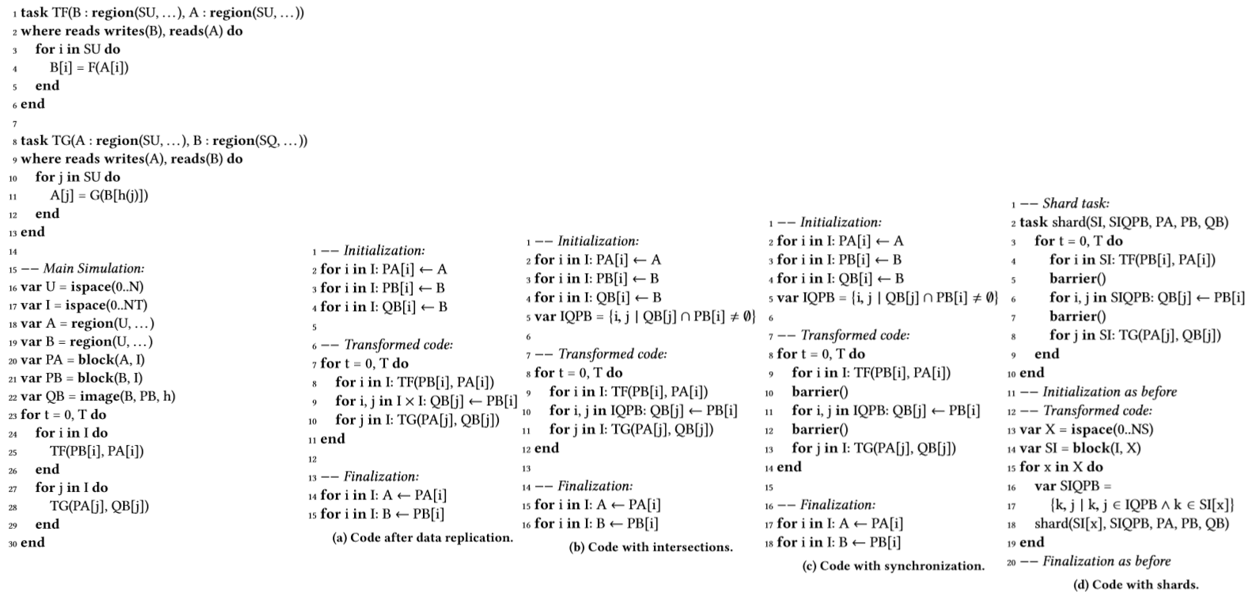
\includegraphics[width=0.90\linewidth]{images/control_replication}
				\caption*{The four stages of control replication as presented in~\cite{Slaughter2017}. \\ $PA$ is a disjoint partition, while $PB$ and $QB$ are aliased and therefore are in need of synchronization.\\ The Tasks TF and TG both write to their first region argument and read their second region argument \\
				$R_1 \leftarrow R_2$ is a shorthand for updating $R_1$ with the values of $R_2$ on the elements $R_1 \cap R_2$ they have in common.}
			\end{figure}

		\end{landscape}

		\newpage

		\begin{landscape}
			\section{Profiling Data generate by Legion Prof for SPH-Regent-SingleR}
			\label{app:SPH-Regent-SingleR-Prof}
			\pagestyle{empty}%

			\begin{figure}[H]
				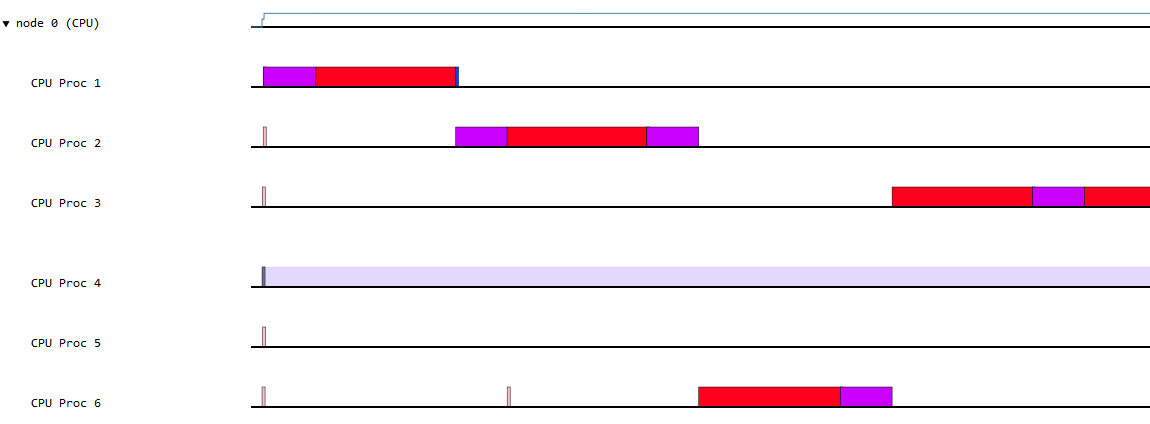
\includegraphics[width=0.95\linewidth]{images/SPH-Regent-Partitioning-Prof}
				\caption*{Excerpt of the profiling data generated by Legion Prof for SPH-Regent-SingleR. Due to tasks being executed on a single region, the program is executed in a sequential fashion. However this does not mean that it is executed in a single thread or on a single processor. In this particular run Processor 4 executed the main loop (light blue) while the tasks launched by the main loop were scheduled randomly onto other processors available. The third stage of the algorithm is not shown on this time scale, as it is too short running to be seeable on this zoom level.}
			\end{figure}

		\end{landscape}

		\newpage

		\begin{landscape}
			\section{Task Dependencies in SPH-Regent-Partitioning}
			\label{app:SPH-Regent-Partitioning-SPY}
			\pagestyle{empty}%

			\begin{figure}[H]
				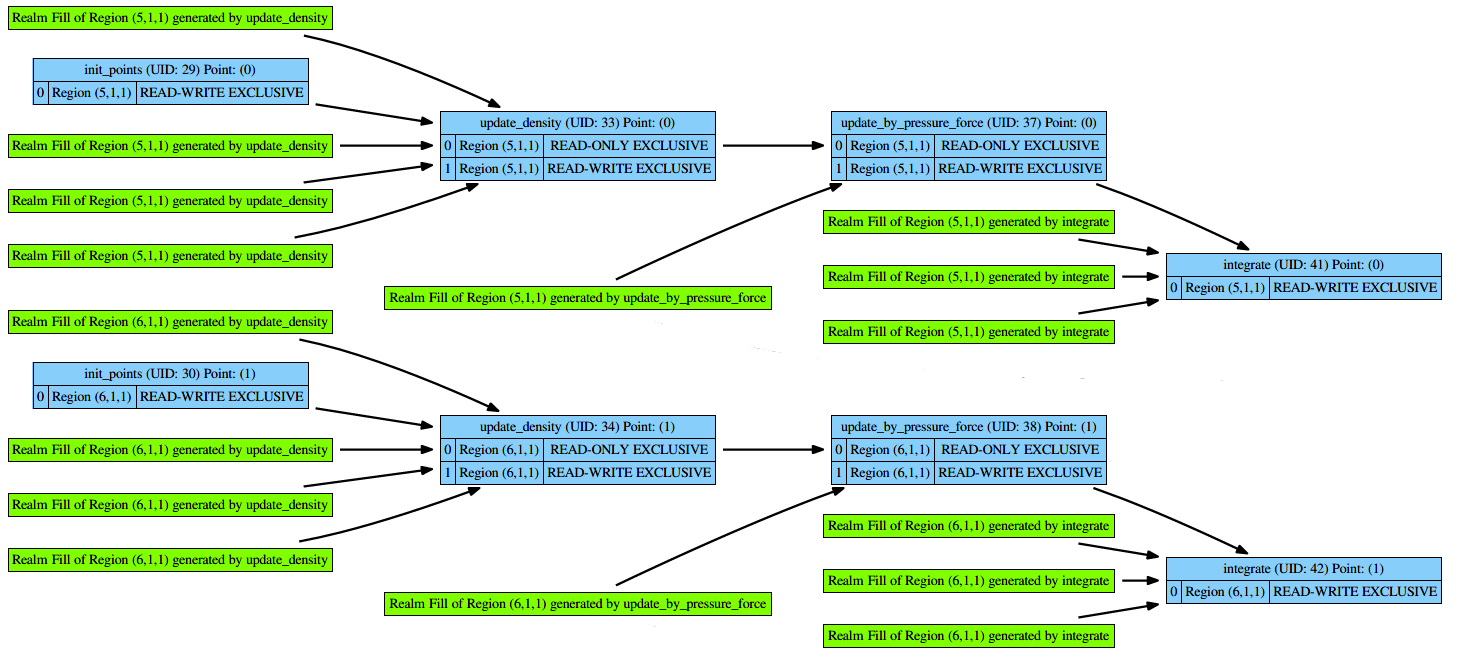
\includegraphics[width=0.95\linewidth]{images/SPH-Regent-Partitioning_SPY}
				\caption*{Excerpt of the task dependency graph generated by Legion Spy for SPH-Regent-Partitioning for task launches on two equal sized partitions of the particle data structure during one iteration of the main loop. The fill operations colored in green are deferred field initalizations generated by Regents \lstinline{fill()} operations. Task launches are colored blue.}
			\end{figure}

		\end{landscape}

		\newpage

		\begin{landscape}
			\section{Task Dependencies in SPH-Regent-Implicit}
			\label{app:SPH-Regent-Implicit-SPY}
			\pagestyle{empty}%
			\begin{figure}[H]
				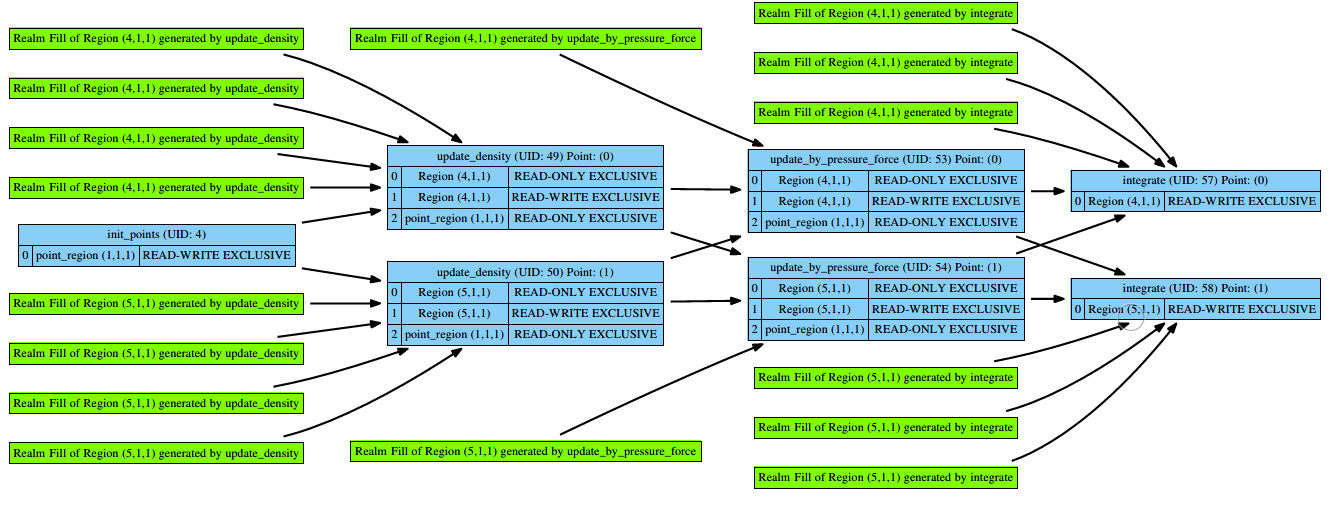
\includegraphics[width=0.95\linewidth]{images/SPH-Regent-Implicit_SPY}
				\caption*{Excerpt of the task dependency graph generated by Legion Spy for SPH-Regent-Implicit for task launches on two equal sized partitions of the particle data structure during one iteration of the main loop. The fill operations colored in green are deferred field initalizations generated by Regents \lstinline{fill()} operations. Task launches are colored blue.}
			\end{figure}
		\end{landscape}
		\newpage
		\begin{landscape}
			\section{Profiling Data generated by Legion Prof for SPH-Regent-Implicit}
			\label{app:SPH-Regent-Implicit-Prof}
			\pagestyle{empty}%

			\begin{figure}[H]
				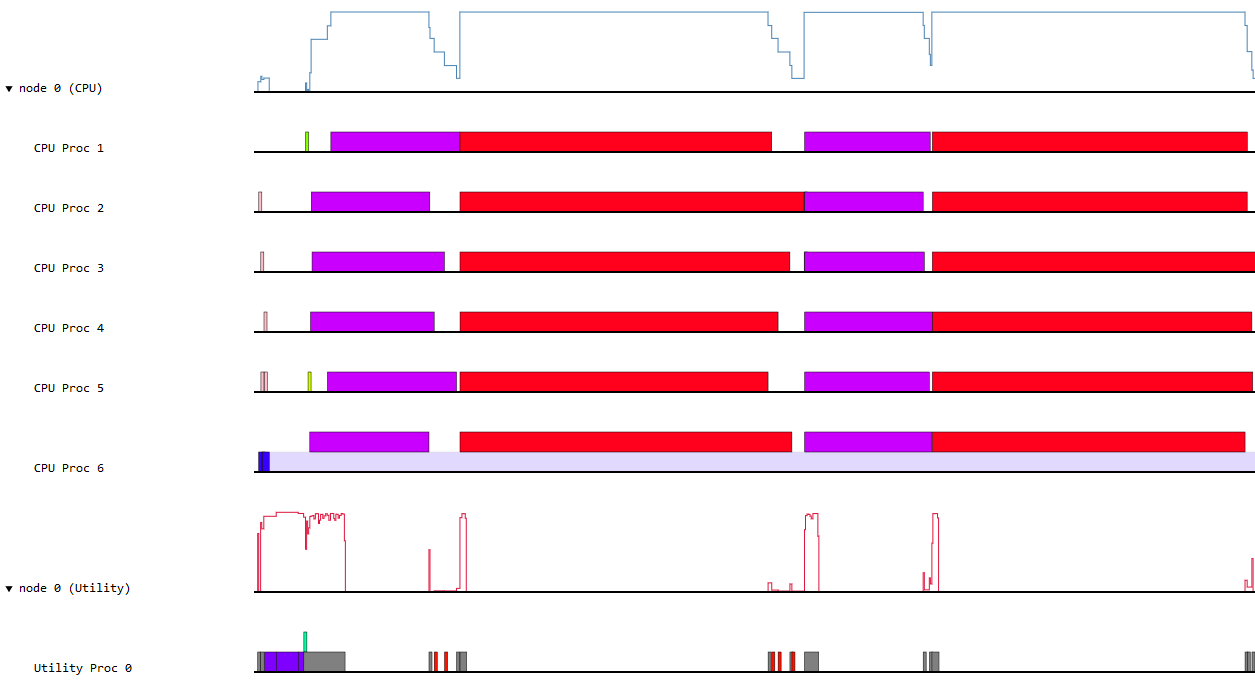
\includegraphics[width=0.88\linewidth]{images/SPH-Regent-Implicit-Prof}
				\caption*{Excerpt of the profiling data generated by Legion Prof for SPH-Regent-Implicit launched with six equally sized partitions. The third stage of the algorithm isn't shown on this time scale, as it is too short running to be seeable on this zoom level. }
			\end{figure}

		\end{landscape}

\end{appendices}

% \addappheadtotoc



\end{document}
% End of document.